

\part{Siebenmann's Theorem}\label{part2}

\chapter{}

\markboth{\thepart. Siebenmann's Theorem}{}

\thispagestyle{plain}

\setcounter{section}{0}
\section[The Assumption of simple-connectedness...]{The Assumption of simple-connectedness in the browder-novikov
  theorem}\label{chap2:sec1}\pageoriginale %% 1


In this  section we will illustrate by examples that simple
connectedness of $X$ and condition (iii) are essential for the
validity of Theorems \ref{chap1:thm2.1} of Part \ref{part1}. We first
construct a compact, 
connected combinational manifold $Y$ of dimension 12 with $\pi_1 (Y) =
0$ and satisfying condition (ii) of Theorem \ref{chap1:thm2.1} which however is not
of homotopy type of any close $C^\infty$ manifold. Since $Y$ is an
orientable $(\pi_1 (Y) = 0)$ compact manifold condition (i) is
automatically satisfied. This example thus illustrates that condition
(iii) of theorem \ref{chap1:thm2.1} (part \ref{part1}) is not
redundant. Let $k$ be any integer 
$\geq 1$ and $\pi^k S^1$ the cartesian product of $k$ copies
of the circle. We will show that $X = Y \times \pi^k  S^1$
satisfies condition (ii), and in case $k$ is divisible by 4 satisfies
condition (iii) as well. However form Siebenmann's Theorem (which will
be stated later) it follows that $X$ is not of the homotopy type of
any closed $C^\infty$ manifold.  

\subsection{}%%% 1.1
The symmetric $8 \times 8$ matrix given below is a unimodular matrix
of signature 8.  

\begin{equation*}
\begin{pmatrix}
2 & 1 & 0 &  0 &  0 & 0 & 0 & 0 \\
1 & 2 & 1 &  0 & -1 & 0 & 0 & 0 \\
0 & 1 & 2 &  1 &  0 & 0 & 0 & 0 \\
0 & 0 & 1 &  2 &  1 & 0 & 0 & 0 \\
0 & -1 & 0 &  1 &  2 & 1 & 0 & 0 \\
0 & 0 & 0 &  0 &  0 & 1 & 2 & 1 \\
0 & 0 & 0 &  0 &  0 & 0 & 1 & 2
\end{pmatrix}
\end{equation*}

Denote\pageoriginale the $(i, j)$ th entry of this matrix by
$C_{ij}$. It is known 
that one can choose $C^\infty$ imbeddings $f_i : S^5 \times 0 \to b
D^{12} = S^{11} (i = 1, \ldots, 8)$ with disjoint images such that the
linking number $L (f_i (S^5 \times 0), f_j (S^5 \times 0))$ of $f_i
(S^5 \times 0)$ and $f_j (S^5 \times 0)$ in $b D^{12} $ for $i \neq j$
are $C_{ij}$. Moreover, for each $i$ we can choose $f_i$ so that
$\equiv$ a differentiably imbedded disk $D'^6_i$ in $D^{12}$ which
bounds $f_i (S^5 \times 0)$. A tubular neighbourhood of $f_i (S^5)$ in
$b D^{12}$ can be got as the restriction of a tubular neighbourhood of
$D'^{6}_i$ in $ D^{12}$. In otherwords $\equiv  C^\infty$ imbeddings
$g_i : D^6 \times D^6 \to D^{12}$ such that $g_i (S^5 \times D^6)
\subset b
D^{12}$, $g_i (S^5 \times 0 = f_i)$ and $D'^6_i = g_i (D^6 \times 0)$. We
can choose these $g_i$ such that $g_i(S^5 \times D^6)$ are pair-wise
disjoint in $b D^{12}$. Let $\wedge : S^5 \to S0_6$ be a $C^\infty$
map representing the element $\partial i_6 \in  \pi_5 (S0_6)$
where $\partial i_6 \in \pi_6 (S^6)$ is a generator and $\lambda$
is the boundary homomorphism in the exact sequence $\pi_6 (S^6) \to
\pi_5 (S0_6) \to \pi_5 (S0_7)$ corresponding to the fibration $S0_7 /
S0_6 = S^6$. Let $ \varphi _i : S^5 \times D^6 \to b D^{12}$ be
defined by $\varphi_i (x, y) = g_i (x, \alpha (x) y)$. Let $D_i^6
\times D^6_i (i = 1, \ldots 8)$ be eight disjoint copies of $D^6
\times D^6$ and let $S^5_i \times D^6_i$ be the submanifold $S^5
\times D^6$ of $D^6_i \times D^6_i$. Let $W^{12} = D^{12} +
(\varphi^6_1) + \cdots + (\varphi^6_8)$ be the compact $C^\infty$
manifold with boundary got from the disjoint union $D^{12} U (U_i
D^6_i \times D^6_i)$ by identifying points of $S^5_i \times D^6_i$
with their images under $\varphi_i$ and then rounding off the
corners. We claim that $W^{12}$ is a manifold with boundary, with $H_6
(W^{12})$  free of rank 8 and having the given matrix as intersection
matrix for a suitable choice of a basis for $ H_6 (W^{12})$. In
$W^{12}$ the image of $D^6_i \times 0$ also a disk bounding $f_i (S^5
\times 0)$ and $\sum^6_i = D'^6_i U(D^6_i \times 0)$\pageoriginale is a
differentiably imbedded sphere in $W^{12}$ whose normal bundle
corresponds to the element $ \partial i_6 \in \pi_5
(S0_6)$. The classes  corresponding to $\sum^6_i$ form a basis for
$H_6 (W^{12})$ since the classes corresponding to $D^6_i \times 0$
form a basis for $H_6 (W^{12}, D^{12})$. The intersections of
$\sum^6_i$ and $\sum^6_j$ in $W^{12}$ are precisely those of $D'^6_i$
and $D'^6_j$ in $D^{12}$ which by definition are the linking numbers
$L (f_i (S^5 \times 0), f_j (S^5 \times 0))$. Hence $\sum^6_i
. \sum^6_j = C_{ij}$ for $i \neq j$. Also if $k_* : \pi_5 (S0_6) \to
\pi_5 (S^5)$ is the map induced by $\varphi \xrightarrow{k} x_\circ. \rho
( x_\circ$ a fixed element in $S^5$) of $S0_6$ in $S^5$ then it is known
that $k_* \partial \iota_6 = \pm 2 \iota_5$ ($i_5$ a generator for
$\pi_5 (S^5)$). Also $k_* (\partial \iota_6)$ is precisely the Euler
class of the normal bundle of each $\sum^6_i$ in $W^{12}$, and this as
we have seen already (Refer to proof of Lemma \ref{chap1:lem5.6}, Part
\ref{part1}) is the self 
intersection $\sum^6_i \cdot \sum^6_i$ times a generator of $\pi_5
(S^5)$. Thus by proper choice of $\iota_6 \in \pi_6 (S^6)$ we see
that $\sum^6_i \cdot \sum^6_i$ can be made equal to 2. Since the matrix we
started with is a unimodular matrix it follows that the boundary
$\partial W$ is a homotopy sphere \cite{c2:key12}. Hence by Smale  \cite{c2:key10} $W$ is
actually a combinatorial $S^{11}$. By attaching the cone over $S^{11}$
to $W$ by a PL-isomorphism we get a closed combinatorial manifold
$Y^{12}$. Clearly $W$ is 5-connected and since $Y^{12}$ is got by
attaching a $12$-cell to $W$ it follows that $Y$ is also 5-connected
and that $H_6 (W) \simeq H_6 (Y^{12})$ under the map induced by the
inclusion $W \to Y$. It follows that $Y$ is a 5-connected
combinatorial manifold of dimension 12, having the given matrix as
intersection\pageoriginale matrix for a suitable choice of basis for
$H_6 (Y)$. 

\setcounter{lemma}{1}
\begin{lemma}\label{chap2:lem1.2} %lemma 1.2
$Y$  is not homotopy type of any compact $C^\infty$ manifold. 
\end{lemma}

\begin{proof}
For if $Y$ were of the homotopy type a compact $C^\infty$ manifold
there should exist classes $p_i H^{4i} (Y; \mathbb{Z}) (i = 1, 2, 3)$
such that $\{L_3 (p_1, p_2, p_3) \}\break [Y] = \left\{\dfrac{1}{3^3. 5.7}
(62p_3 - 13p_2 p_1 + 2p^3_1) \right\} [Y] = 8$.  Since $ H^4 (Y;
\mathbb{Z}) = 0 $ and $H^8 (Y; \mathbb{Z}) = 0$ the above implies
that $\exists$ a class $p_3 \in H^{12} (Y ; \mathbb{Z}) \simeq
\mathbb{Z}$  such that $\dfrac{1}{3^3. 5. 7} 62p_3 [Y] = 8$. This in
turn means the existence of an integer $ \ell_3$ such that $62 \ell_3
= 3^3 .5. 7. 8$. This is impossible since the prime 31 does not divide
$3^3 .5 .7.8$.  
\end{proof}

\begin{lemma}\label{chap2:lem1.3} %lemma 1.3
 Let $\xi$ be the tr ivial line bundle over $Y$. Then for the Thom
  space $T(\xi)$ of $\xi$ the homology $H_{13} (T (\xi))$ has a
  spherical generator. 
\end{lemma}

(This observation is due to A. Vasqez.)

\begin{proof}
$Y$ is a 5-connected polyhedron with $H_6 (Y)$ free abelian of rank
  $8, H_{12} (Y) \simeq \mathbb{Z} ; H_j (Y) =0$ for all other $j \geq
  1$. Thus a `homology decomposition' \cite{c2:key2} for $Y$ will be $(S^6 V
  \ldots V S^6 ) \underset{h}{U} E^{12}$ where the wedge is a 8 fold wedge and to
  it is attached a 12-cell by means of a map $h : S^{11} \to S^6
  \ldots V S^6$ representing the so called $k$-invariant or the dual
  Postnikov invariant. The Thom space $T(\xi)$ of $\xi$ is homotopy
  equivalent to the suspension $\sum (Y U \text{ `$a$'})$ of the disjoint union
  of $Y$ and a point `$a$'. Hence $T(\xi) \sim  S^1 V ( S^7 V \ldots V S^7)
  \underset{g}{U} e^{13}$ (we use `$\sim$' to mean homotopy equivalence) where $g :
  S^{12} \to S^1 V S^7 V \ldots V S^7$ is some map. It is known that
  $\pi_{12} (S^7) = 0$ \cite{c2:key4}. By a\pageoriginale theorem of Hilton
  \cite{c2:key3} it follows that 
  $\pi_{12} (S^1 V S^7 V \ldots VS^7 ) =0$. This shows that $g$ is
  homotopically trivial and hence $T(\xi) \sim S^1 V (S^7 V \ldots
  VS^7)VS^{13}$. The inclusion of $S^{13}$ in $S^1 V(S^7 V \ldots
  VS^7) VS^{13}$ followed by a homotopy equivalence $f : S^1 V(S^7 V
  \ldots VS^7) VS^{13} \to T(\xi)$ represents a generator of $H_{13}
  (T(\xi))$. 
\end{proof}

\begin{lemma}\label{chap2:lem1.4} %lemma 1.4
Let $V$  be a closed, connected, orientable combinatorial manifold
satisfying condition  (ii)  of Theorem \ref{chap1:thm2.1} (Part
\ref{part1}). Then $V \times 
S^1$ also satisfies condition (ii). If  $\dim. V = 4d -1$ then $V S^1$
also satisfies condition (iii). 
\end{lemma}

\begin{proof}
Let $\dim V =n$ and let $\xi^k$ be an orientable vector bundle of rank
$k$ on $V$ with $H_{n+k} (T (\xi)) \simeq \mathbb{Z}$ with a spherical
generator, say represented by the map $f : S^{n+k} \to T
(\xi)$. Choose any orientable vector bundle $\eta$ of rank $\ell$ over
$S^1$ with a spherical generator for $H_{\ell +1} (T (\eta )) \simeq
\mathbb{Z}$ represented by $g : S^{\ell +1} \to T (\eta)$. Such a
bundle exists since $S^1$ is a $C^\infty$ manifold. (In fact the
trivial line bundle itself satisfies this condition). Let $\zeta
\times \eta$ be the cartesian product bundle on $V \times
S^1$. Choosing fixed Riemannian metrics for $\zeta$ and $\eta$ denote
the associated unit disk bundles by $A_\xi$ and $A_\eta$ and let
$\dot{A}_\xi$ and $\dot{A}_\eta$ be the boundaries of $A_\xi$ and $A_\eta$
respectively. Then $T(\xi ) = A_\xi / \dot{A}_\xi$ and $T (\eta) = A_\eta /
\dot{A}_\eta$. For the bundle $\xi \times \eta$ with the cartesian
product Riemannian metric we have $A_{\xi \times \eta} = A_\xi \times
A_ \eta$ and $ \dot{A}_{\xi \times \eta} = A_\xi \times \dot{A}_\eta \cup
\dot{A}_\xi \times A_\eta$. Choosing the respective points at $\infty$ as
base points in $T(\xi)$ and $T (\eta)$ let $T (\xi) \# T(\eta) =
\dfrac{T(\xi) \times T (\eta )}{T (\xi) V T (\eta)}$. The canonical
projections $\varepsilon_\xi : A_\xi \to T(\xi)$ and $\varepsilon_\eta :
A_\eta \to T (\eta)$ yield the map $\varepsilon_\xi \times \varepsilon_\eta
: A _\xi \times A_\eta \to T (\xi) \times T (\eta)$.\pageoriginale If
$p : T (\xi) 
\times T(\eta) \to T (\xi ) \# T (\eta)$ is the canonical map then $po
(\varepsilon_\xi \times \varepsilon_\eta) :  A_\xi \times A_\eta \to T
( \xi / \# ) Tm$ yields a $(1-1)$ onto map of $\dfrac{A_\xi \times
  A_\eta}{A_\xi \times \dot{A}_\eta \cup \dot{A}_\xi \times A_\eta} \to T (\xi) \#
T (\eta)$. The compactness of the spaces involved shows that the map $T
( \xi \times \eta) \to T (\xi ) \# T (\eta)$ thus obtained is a
homeomorphism. Clearly the map $f \# g : S^{n+k} \# S^{\ell +1} =
S^{n+1+k+\ell} \to T (\xi) \# T (\eta )$ represents a generator of
$H_{n+1+k+\ell} (T (\xi \times \eta))$. 
\end{proof}

 Suppose $n = 4d - 1$. Choose a basis $X_1, \ldots, X_r$ for $ H^{2d
   -1}(V; \mathbb{Q})$. By Poincare duality $\exists$ a basis $Y_1,
 . , Y_r$ for $ H^{2d}(V ; \mathbb{Q})$ such that $X_i$.  $Y_j =
 \delta_{ij}$. Then for  $H^{2d} (V \times S^1 ; \mathbb{Q})$ the
 elements $X_1 \otimes s, \ldots, X_r \otimes s ; Y_1 \otimes 1,
 \ldots, Y_r \otimes 1$ where $s \in H^1 (S^1, \mathbb{Q})$
 is a generator form a basis. With respect to this basis the
 intersection matrix is
 $2d \overbrace{
\begin{cases}
 \left( \begin{smallmatrix} 
0 & I\\
I & 0 
\end{smallmatrix}
\right)
 \end{cases}}^{2d}$. Hence the signature of the
 manifold $V \times S^1$ is 0. Choosing $ \eta$ to be the trivial line
 bundle on $S^1$ we have $L_d (\bar{p}_1 (\xi \times \eta ), \ldots,
 \bar{p}_d ( \xi \times \eta)) [ V \times S^1] = L_d (\bar{p}_1 (\xi)
 \otimes 1, \ldots, \bar{p}_d (\xi ) \otimes 1) [ V \times S^1] = 0$. 

It follows from Lemmas \ref{chap2:lem1.3} and \ref{chap2:lem1.4} that
$ X^{12 +k} = Y^{12} \times 
\pi^{k} S^1$ satisfies conditions (i) and (ii) of Theorem
\ref{chap1:thm2.1} (Part \ref{part1})
and also (iii) in case $ k \geq 1$ is divisible by 
4. From Siebenmann's Theorem stated below and Lemma  \ref{chap2:lem1.2} it will
follow that none of the manifolds $X^{12+k} (k \geq 0)$ is of the
homotopy type of a compact $ C^\infty$ manifold. 

Let $\pi$ be any multiplicative group and $\mathbb{Z} (\pi)$ the group
ring of $\pi$ over $\mathbb{Z}$. Two finitely generated projective
$\mathbb{Z} (\pi)$-modules $P_1$ and $P_2$ are said to be equivalent
if $\exists$ finitely generated free $\mathbb{Z} (\pi)$
-modules\pageoriginale 
$F_1$ and $F_2$ with $P_1 \oplus  F_1 \simeq F_2 \oplus F_2$. The set
of equivalence classes of finitely generate a projective modules is
denoted by $\tilde{K}_\circ (\mathbb{Z} (\pi))$; it is an abelian group under
the operation induced by the direct sum operation on projective
modules.  

\setcounter{theorem}{4}
\begin{theorem}[Siebenmann]\label{chap2:thm1.5} %Theorem 1.5
 Let $X$ be a finite complex such that $X \times S^1$ is
  of the homotopy type of a compact, connected, $C^\infty$ manifold $V^{n+1}$
  without boundary of dimension $n+1$ with $ n \geq 5$. Suppose
  $\mathbb{Z} (\pi)$ is Noetherian and that $\tilde{K}_\circ
  (\mathbb{Z}(\pi)) = 0$ where $\pi =  \pi_1 (X)$. Choosing a homotopy 
  equivalence $\theta : V \to X \times S^1$ and denoting the
  projection onto the second factor $X \times S^1 \to S^1$ by $p_2$
  let $W$ be the covering of $V$ got as the pull back of the covering
  $\mathbb{R} \xrightarrow{(Exp 2 \pi i)} S^1$ by means of the map
  $p_2 . \theta : V \to S^1$. Then $W$ with the natural
  differential structure it acquires as a covering manifold of $V$, is
  diffeomorphic to $N^n \times  \mathbb{R}$ with $ N = N^n$ a compact
  $C^\infty$ manifold without boundary, of dimension $n$. 
\end{theorem}

\begin{remark*}
As $W$ is of the homotopy type of $X\times \mathbb{R}$ or $X$ it
follows that $X$ is of the homotopy type of $N$. If $\pi$ is free
abelian of rank $\ell < \infty$ we have  $\mathbb{Z}(\pi)_\simeq
\mathbb{Z} [x_1, \ldots, x, x_1^{-1}, \ldots, x_\ell^{-1}]$ where $x_1,
x_2, \ldots x_\ell$ are $\ell$-indeterminates over  $\mathbb{Z}$ and in
this case  $\mathbb{Z} (\pi)$ is Noetherian and $\tilde{K}_\circ
\mathbb{Z} (\pi)) =0$. It is now clear that none of the manifolds
$X^{12+k} = Y^{12} \times \pi^{k} S^1$ is of the homotopy
type of any compact $C^\infty$ manifold without boundary. 
\end{remark*}

The theorem remains true if we drop the assumption that
$\mathbb{Z}(\pi)$ is Noetherian. We give some more details on this in 
\S \ref{chap2:sec3}. The assumption $\tilde{K}_\circ  \mathbb{Z}
(\pi))$ is however 
essential. An example of a group with\pageoriginale $\tilde{K}_\circ
\mathbb{Z} (\pi)) \neq 0$  is the cyclic group or order 23. (See
D.S. Rim \cite{c2:key9}).  

The rest of Part \ref{part2} deals with the Proof of Theorem
\ref{chap2:thm1.5}. Let $ f : V 
\to S^1$ pe a $C^\infty$ approximation to $p_2 \circ \theta$ with $f \sim
p_2  \circ \theta : V \to S^1$ (we use `$\sim$' to mean `homotopic'). We
denote the map $Exp ( 2 \pi i) : \mathbb{R} \to S^1$ by $q$ and let
$p : W \to V$ denote the covering mapping. By definition $W$ is the
inverse image of the covering $q:  \mathbb{R} \to S^1$ by means of
the map $p_2 \circ \theta : V \to S^1$. Since $f \sim p_{2} \circ \theta
\exists$ a map $F: W \to \mathbb{R}$ making the following diagram
commutative. Moreover $F$ is $C^\infty$. 
\begin{center}
\begin{gather*}
\xymatrix{
W \ar[r]^F \ar[d]_p & \mathbb{R} \ar[d]_{q} \\
V \ar[r]^f & S^1
} \\
\centerline{\bf Diagram 1}
\end{gather*}
\end{center}


By Sard's Theorem $\exists$ a regular value $a \in S^1$ for
$f$ and without loss of generality we can assume $1 \in S^1$
to be a regular value for $f$. Then any integer is a regular value of
$F$. 

\section[The existence of arbitrary small...]{The existence of arbitrary small 0 and\hfil\break 1-Neighbourhood of
  `$\infty$' and `$-\infty$'}\label{chap2:sec2} %%% 2

\begin{definition} %definition 2.1
A $C^\infty$ sub-manifold $M = M^{n+1}$ of dimension $n+1$ with
boundary $b M$, of $W$ is said to be a 0-nbd of $\infty$ (respy
``$-\infty$'') if  
\begin{enumerate}[(1)]
\item $M$ is a closed subset of $W$

\item $\exists$ integers $m_1 < m_2$ with $F^{-1}[ m_1, \infty )
  \supset M \supset F^{-1}[M_2, \infty)$ 

$\left\{ \text{ respy } F^{-1}(
    -\infty, M_1] \subset M \subset F^{-1}(-\infty, M_2]\right\}$ 

\item  $b M$ is\pageoriginale compact; $M$ and $b M$ are connected.
\end{enumerate}

$M$ is said to be a $1-nbd$ of $\infty$ (respy ``$-\infty$'') if it
is already a $0- nbd$ of $\infty$ (respy ``$-\infty$'') and the maps
$\pi_1 (b, M) \to \pi_1 (M)$, $\pi_1(M) \to \pi_1(W)$ induced by the
respective inclusions are isomorphisms. 
\end{definition}

\begin{definition}%defini 2.2
By the statement  ``arbitrary small 0 (or 1)-$nbds$ of $\infty$
(respy $-\infty$)'' we mean that given any compact set $K \subset W$
$\exists$ a 0 (or 1) $-nbd$ $M$ of $\infty$  (respy $-\infty$) with $M
\subset W - K$. 

Let $J$ denote an infinite cyclic group and let $x$ be a generator of
$J$. The Deck transformation group of the covering $\mathbb{R}
\xrightarrow{q} S^1$ can be identified with $J$ with $x$ acting as the
homeomorphism $r \to r + 1$ of $\mathbb{R}$ onto itself. Since $W
\xrightarrow{p} V$ is the pull back of the covering space $\mathbb{R}
\xrightarrow{q} S^1$ the Deck transformation group of the covering $W
\xrightarrow{p} V$ is also $J$ and we denote the homeomorphism of $W$
which corresponds to the generator $x$ by $\alpha$. 
\end{definition}

\setcounter{lemma}{2}
\begin{lemma}\label{chap2:lem2.3}%lemma 2.3
Let $\sigma$ be any are in $V$  and $w_\circ \in W$ any point with $
p(w_\circ) = \sigma (0)$.  Let $\tau^{w_\circ}$ be the unique lift of
$\sigma$ such that $\tau^{w_\circ}(0) = w_\circ$.The variation $\Max_{t, t'
  \in [0, 1]} | F \tau^{w_\circ}(t) ---- F \tau^{w_\circ} (t')|$ of
$F$ on $\tau^{w_\circ}$ 
depends only on $\sigma$ and not on the lift $w_\circ$ of $\sigma (0)$. 

This quantity which depends only on $\sigma$  we refer to as the
``variation of $F$ on $\sigma$'' and denote it by $V_F (\sigma)$. 
\end{lemma}

\begin{proof}
Suppose $w_\circ'$, is any other element of $W$  with $p(w_\circ') =\sigma
(0)$, then $w_\circ' = \alpha^{k} w_\circ$, for some integer $k$. The unique
lift $\tau^{w'_\circ}$ of such that $\tau^{w'_\circ} = w'_\circ$ is given by
$\tau^{w'_\circ} (t) = \alpha^{k} \tau^{w_\circ} (t)$.  Because of
the\pageoriginale commutativity of diagram 1 we have  
$$
F \tau^{w'_\circ} (t) = k + F \tau^{w_\circ} (t) 
$$
for all $t \in[0, 1]$. The lemma follows.
\end{proof}

\begin{lemma}\label{chap2:lem2.4}%%%2.4 
There exists a constant $C > 0$ such that any two points of $V$ can be
joined by means of an are $\sigma$ such that the variation $V_{F}
(\sigma)$ of $F$ on $\sigma$ is less than $C$. 
\end{lemma}

\begin{proof}
For any $v \in V$ $\exists$ an arcwise connected  open $ndb$ $U_{v}$
of $v$ in $V$ such that $p^{-1} (U)_v$ decomposes into a disjoint
union of open sets $\{ W^{j}_{v} \}$ each of which gets mapped
homeomorphically onto $U_{v}$ by the restriction of $p$. We can choose
another arcwise connected open set $U'_{v}$ containing $v$ such that
$\bar{U}'_{v} \subset U_{v}$. Then each of the sets 

$W_{v}'^{j} = W_{v}^{j} \cap p^{-1}(U_{v}')$  gets mapped
homeomorphically by $p$ onto $U_{v}'$ and $W_{v}'^{j} =
p^{-1}(U_{v}')\cap W^{j}_{v}$ is compact since $\bar{U}'$ is compact,
being a closed subset of the compact space $V$. The argument used in
lemma \ref{chap2:lem2.3} can be used to show that $\underset{w, w^1
  \in \bar{w}' j}{\Max}| 
F(w) - F(w^1) |$ is finite and depends  only on $U'$ (finiteness being
a consequence of the compactness of $\bar{W'}^j $).  We may call the
above quantity the variation of $F$ on $ U'$ or $\bar{U}'$.
Compactness of $V$ implies the existence of a finite number of sets
$U_{v_{1}}', \ldots , U_{v_{r}}'$  covering $V$. Writing $U_i'$ for
$U_{v_{i}}'$ and denoting the variation of $F$ on $U_i'$ by $C_i$ let
$C$ be any constant $ > C_1 + \cdots  + C_r$. Then $C$ satisfies the
requirement of the Lemma. For if $v_{\circ}, v_{1}$ are  any two points
of $V$, since $V$ is arcwise connected we can find distinct indices
$j_{1}, \ldots , j_s$, in $1, 2, \ldots, r$ such that $v_{\circ}\in
U'_{j_1}$ and  $v_{1} \in U'_{j_{\ell}}$ and $U'_{j_{\mu}} \cap
U'_{j_{\mu+1}} \neq \not\phi$.\pageoriginale Choosing point $v'_{\mu}
U'_{\mu +1}$ and 
joining $v_{\circ} to v_{1}'$ by an arc in $U_{j_{1}} ; v_{1}'$ to
$v_{2}'$ by an arc in $U'_{j_{2}}$ and so on  we get an are $\sigma$
joining $v_{\circ}$ to $v_{1}$ such that $V_{F} (\sigma) \leq C_{j_{1}} +..+
C_{j} < C$. 
\end{proof}

\begin{lemma}\label{chap2:lem2.5}%lemma 2.5
a constant $ \alpha > 0 $ with the following property: For every $v
\in V$ $\exists$ a loop $\theta _{v}$ at $v$ in $V$ such that the
loop $f \theta _{v}$ represents the positive generator of $ \pi_{1}
(S^{1}, f(v))$, and $V_F (\theta )< d$.  
\end{lemma}

\begin{proof}
Choose a point $v_\circ \in V$ and any loop $\theta_{v_\circ}$ at $v_\circ$
such that $f \theta_{v_\circ}$ represents the positive generator of
$\pi_1 (S^1, f(v_\circ))$. Let $e$ be the variation of $F$ on
$\theta_{v_\circ}$ and $C > 0$ the constant of Lemma \ref{chap2:lem2.4}. Then $d = 2C
+ e$ satisfies the requirement of Lemma \ref{chap2:lem2.5}. For given any $v \in V
\exists$ a path $\sigma^{v}$ in $V$ such that $\sigma^{v}(0) = v$,
$\sigma^{v}(1) = v_\circ$ and $V_{F} (\sigma^{v}) < C$. If we define
$\theta _{v}$ for any $v \neq v_\circ$ by $\theta _{v} = \sigma^{v}
\theta_{v_\circ} (\sigma )^{v-1}$ then clearly  
$ f{\theta}_{v}$ represents the positive  generator of $\pi_{1}
((S^{1}), f(v))$ and $V_{F}(\theta )_{v} < C + e + C = 2C + e = d$. 
\end{proof}

According to our choice of $d$ we have $d > c$.

\begin{lemma}\label{chap2:lem2.6}%lemma 2.6
Let $w$ be any element of $F^{-1} [\ell + d, \infty)$ with $\ell$ any
  real number and $v = p (w)$.  For any integer $k \geq 0$ let
  $\tau_{k}$ be the unique lift of $\theta^{k}_{v}$ satisfying
  $\tau_{k}(0) = w$. Then the path $\tau_{k}$ lies in
  $F^-1[\ell,\infty)$ and $F (\tau_{k}(1)) = k + F (w)$. 
\end{lemma}

\begin{proof}
The $ F(\tau_{k}(1)) = k+F(w)$ follows from the fact that $f \circ
\theta^{k}_{v}$ represents the element $k.$ ($+$ ve generator) of
$\pi_{1}(S^{1} f(v))$. The $\tau _{k}$ lies in $F^{-1}[\ell, \infty)$
  is proved by induction on $k$. For $k = 0$ there is
  nothing\pageoriginale to prove. Assume $k \geq 1$ and the lemma
  valid for $(k - 1)$ instead of $k$. Let $\mu$ be the lift of
  $\theta_{v}$ with initial point $\mu (0) = \tau_{k-1}(1)$. Then
  $F_{\mu}(0) = (k-1) + F(w) \geq (k-1) + \ell + d$. Since the
  variation of $F$ on $\theta_{v} < d$ we have $F \mu (t)\geq (k-1) +
  \ell \forall t \in [0, 1]$. Since $k \geq 1$ this implies  $F \mu
  (t)\geq \ell$. Now $ \tau_{k}$ is precisely the product
  $\tau_{k-1}. \mu$ and whenever $t \leq \dfrac{1}{2}$, $F \tau_{k}
  (t) = F \tau_{k-1} (2t) \geq \ell$ (by induction hypothesis) and if
  $t \leq \dfrac{1}{2}$, $F \tau_{k}(t) = F \mu (2t-1) \geq (k-1) +
  \ell$ (by what is proved above). This shows that $\tau_{k}$ lies in 
  $F^{-1} [\ell, \infty)$. 
\end{proof}

\setcounter{prop}{6}
\begin{prop}\label{chap2:prop2.7}%proposi 2.7
 There exist arbitrary small 0-neighbourhoods of `$\infty$'
  (resp. $-\infty$) in $W$. 
\end{prop}

\begin{proof}
We prove the assertion for $ \infty$, the proof for ``$-\infty$''
being similar is left out. Let $K$ be any compact subset of
$W$. $\exists$ an integer $\ell$ such that $F^{-1} [\ell, \infty)
  \subset W - K$. Since $\ell$ is a regular value of $F$ we see that
  $F^{-1} [\ell, \infty)$ is a $C^ \infty$ submanifold of $W$, with
    boundary $F^{-1}(\ell)$. Let $d$ be the constant of Lemma \ref{chap2:lem2.5}
    (which as commented earlier has been chosen to be  $> C$ the
    constant of Lemma \ref{chap2:lem2.4})  
\end{proof}

\noindent
\textbf{Claim:} Any two points $w_\circ$, $w_1$ of $F^{-1} [\ell + 2d,
  \infty)$ can be joined by means of a path in $F^{-1} [\ell ,
    \infty)$. 

Let $p(w_\circ) = v_\circ$, $p (w_1) = v_1$. By Lemma
\ref{chap2:lem2.4} $\exists$ an arc 
$\sigma$ in $V$ such that $\sigma (0) = v_\circ$, $\sigma (1) = v_{1}$ and
$V_F (\sigma) < C$.  Let $\tau$ be the unique lift of $\sigma$ with
initial point $\tau(0) = w_\circ$. The $\tau (1)$ and $w_{1}$ are points
on the same fibre of $W$ and hence $F (w_1) = k + F(\tau (1))$ for a
certain integer $k$. It follows that $\sigma^{1} =
\theta^k_{v_\circ}$. $\sigma$ is a path joining $v_\circ$ to $v_1$ in
$V$ whose lift $\tau^1$ with initial point $\tau^{1} (0) =
w_\circ$\pageoriginale satisfies $\tau^1 
(1) = w_1$. We now consider the cases $k\geq 0$ and $k < 0$
separately. Case (i) $k\geq 0$. Since $V_F (\sigma ) < C < d $ and
$F(\tau (0)) = F(w_\circ) \geq \ell + 2d$ it follows that $F(\tau (t)) >
\ell + d$. From Lemma \ref{chap2:lem2.6} we now have $F (\tau^1 (t))
\geq \ell \forall t 
\in [0, 1]$. Case (ii) $k < 0$. The path $(\tau^1)^{-1}$ is the
composition $(\tau_{-k})$. $ \tau^{-1}$ where $\tau_{-k}$ is the lift
of $ \theta^{k}_{v_\circ}$ having as initial point $\tau_{-k}(0) =
w_{1}$. Now, by assumption $F(w_1)\geq \ell + 2d$ and $-k > 0$. From
Lemma \ref{chap2:lem2.6} we see that $\tau_{-k}$ is an arc in $F^{-1} [\ell,
  \infty)$. Since $\tau$ (and hence $\tau^{-1}$ also) is an arc in
  $F^{-1}[\ell + d, \infty)$  we see that $(\tau^1)^{-1} =
    \tau_{-k}.\tau ^{-1}$ is an arc in $F^{-1}[\ell, \infty)$ and
      hence $\tau^1$ too is an $F^{-1}[\ell, \infty)$. 

This completes the proof of the claim. Now it is clear that $F^{-1} 
[\ell, \infty)$ has only one non-compact connected component say $M'$
  and a finite number of compact connected components. Since $M'
  \supset F^{-1}[\ell + 2d, \infty)$ it follows that the boundary
    $bM'$ of $M'$ lies in $F^{-1}[\ell,\infty) - F ^{-1}(\ell + 2d,
      \infty)$ and is therefore compact. If $bM'$ were connected then
      $M'$ itself would be a $0 - nbd$ of $\infty$. Suppose $bM'$ is
      not connected. Choosing a smooth path in $M'$ from one component
      of $bM'$ to another meeting $bM'$ orthogonally and only at the
      end points and removing the interior of a tubular neighbourhood
      of the path we get a connected $C^\infty$ submanifold $M''$ of
      $W$ with  

\begin{figure}[H]
\centering
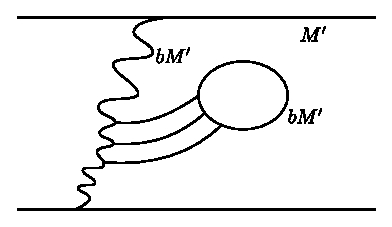
\includegraphics{vol46-fig/fig46-1.eps}
\centerline{\bf Diagram 2}
\end{figure}

$bM''$\pageoriginale compact and $bM''$ having one component less than
$bM'$. Refer 
to Diagram 2. Since there are only a finite number
of components after 
a finite number of such operations we get a connected $C^\infty$
submanifold $M$ of $W$ with $bM$ compact and connected. Further $M
\supset F^{-1} [m,\infty)$ for some integer $m$ since the original
  $M'$ contained $F^{-1} [\ell + 2d, \infty)$. Thus $M$ is a $0 - nbd$
    of $\infty$. 

\setcounter{lemma}{7}
\begin{lemma}\label{chap2:lem2.8}%lemma 2.8
Let $M^{n+1}$ be a $C^\infty$ submanifold of $W^{n+1}$ with boundary
$bM = N$ and let $M$ and $N$ be connected. Let $M$ be a closed subset
of $W$. Suppose the homomorphism $\pi_1 (N) \to \pi_1(W)$ induced by
the inclusion is an isomorphism. This $\pi_1 (M) \to \pi_1 (W)$
induced by the inclusion of $M$ in $W$ is also an isomorphism. 
\end{lemma}

\begin{proof}
Let $i : N \to M$ and $j : M \to W $ be the respective
inclusions. Then $j \circ i : N \to W$ induced an isomorphism $(j
\circ i)_* :
\pi_1 (N) \to \pi_1 (W)$ by our hypothesis. Since $(joi)_* = j_*  \circ i_*$ it
follows that $j_* : \pi_1 (M)\to \pi_1(W)$ is an epimorphism. To show
that $j_* : \pi_1 (M)\to \pi_1 (W)$ is an isomorphism it therefore
suffices to prove that $j_*$ is a monomorphism. Since $\dim M = n+1$
and $n \geq 5$ any element of $\pi_1 (M)$ can be represented by a
$C^{\infty}$ imbedding $\varphi : S^1 \to$ Int $M$ (in fact for this
assertion to be valid it suffices that $n + 1 \geq 3$). Suppose
$\alpha \in \pi _1 (M)$ is such that $j_* (\alpha ) = 0$ and
suppose $\varphi : S^{1}\to$ Int $M$ represents $\alpha$. From
$j_*(\alpha ) = 0$ it follows that $\exists$ a map $h : D^{2}\to W$
extending $\varphi$. Since $\phi (S^1) \cap N = \phi$ we can
approximate $h$ by a $C^{\infty}$ map $\theta : D^2 \to W$ such that
$\theta / S^1=\varphi$ and\pageoriginale $\theta$ is transverse regular
on $N$. Then 
$D^2 \cap \theta^{-1} (N)$ consists of a finite number of disjoint
simple closed curves (each one of them is a $C^\infty$ imbedded $S^1$)
in the interior of $D^2$. Take an inner most curve $C$. Now $\theta |
C \to W$ admits of an extension $\theta : \bigtriangleup \to W$ where
$\bigtriangleup$ is the closed region (inner most) bounded by
$C$. Thus $\theta | C$ represents the trivial elements of $\pi_1(W)$
and $\theta (C)\subset N$. Since $\pi_1 (N)\to \pi_1 (W)$ is an
isomorphism it follows that $\exists $ a map $\lambda : \bigtriangleup
\to N$ with $\lambda | C = \theta | C$. (Refer to diagram 3). Now
using the fact that $N$ is collared in $M$ it is easy to get a map
$\theta' : D^{2}\to W$ with the following properties: 

\begin{figure}[H]
\centering
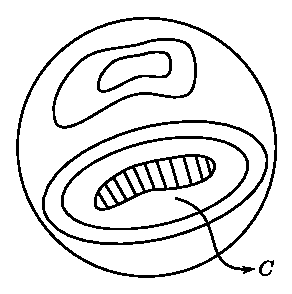
\includegraphics{vol46-fig/fig46-2.eps}
\centerline{\bf Diagram 3}
\end{figure}
\begin{enumerate}[(1)]
\item $\theta' | S^1 = \varphi$

\item $\exists$ a $nbd A$ of $\bigtriangleup$ in $D^2$ with $A$
  disjoint from the curves of $\theta^{-1} (N) \cap D^2$ different
  from $C$ such that $\theta' (A) \cap = \phi$ and  $\theta' | D^2 - A
  = \theta | D^2 - A$. 
\end{enumerate}
For this $\theta'$ we have $\theta'^{-1} (N) \cap D^2$ consisting
precisely of the curves in $\theta^{-1} (N) \cap D^2$ excepting
$C$. Repeating this argument a finite number of times we finally get a
map $\Phi : D^2\to W$ such that $\Phi S^1 = \varphi$ and $\Phi^{-1}(N)
\cap D^2 =\emptyset$. Since $\varphi (S')\subset$ Int $M$ and since $D^2$
is connected we should have $\Phi  (D^2) \subset$ Int $M$, for
otherwise $D^2 \cap \Phi^{-1}$ (Int $M$) and\pageoriginale $D^2 \cap
\Phi^{-1}(W- M)$ will be non void disjoint open sets of $D^2$. This
means that $\alpha \in \pi_1 (M)$ is the zero element and hence
$\pi_1 (M) \to \pi_1 (W)$ is a monomorphism.  
\end{proof}

\setcounter{prop}{8}
\begin{prop}\label{chap2:prop2.9}%%% 2.9
There exist arbitrary small 1-neighbourhoods of ``$\infty$''. 
\end{prop}

In the proof of this lemma we use a result in group theory which we
state below without proof. 

\setcounter{lemma}{9}
\begin{lemma}\label{chap2:lem2.10}%lemma 2.10
Suppose $G$ and $H$ are finitely presentable group and $G
\xrightarrow{h}H \rightarrow 1$ is an exact sequence. Then the Kernel
of $h$ is the normal subgroup in $G$ generated (as a normal subgroup)
by a finite number of elements. 
\end{lemma}

We now go to the proof of proposition \ref{chap2:prop2.9}. We have $\pi_1(W) \simeq
\pi_1 (X)$ and by assumption $X$ is a finite polyhedron. It follows
that $\pi_1 (W)$ is finitely presentable. Let $M'$ with $N' = bM'$  be a
zero neighbourhood of $\infty$ with $M' \subset W-K$. Choosing a base
point $w_\circ \in$ Int $M'$ and a small ``contractible open set 0''
in Int $M'$ as the ``new base point'' we can represent a finite system
of generators $\alpha_1, \ldots, \alpha_r$ of $\pi_1 (W)$ by disjoint
$C^\infty$ imbeddings $\varphi_i : S^1 \to W(i = 1,\ldots r)$ with the
base point of  $S^1$ going into 0. To represent each $\alpha_i$ by a
$C^\infty$ imbeddings we need that $\dim W \geq 3$ and also to get the
imbedding to have disjoint images we need $\dim W \geq 3$. But
hypothesis $\dim W \geq 6$. By choosing $w_\circ$ properly we can assume
that $\varphi_i (S^1) \subset$ Int $M'$ for every $i$. 

\begin{figure}[H]
\centering
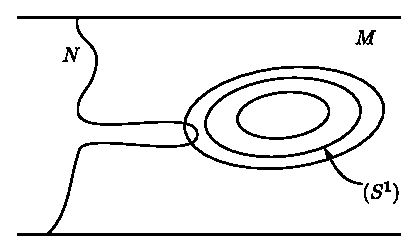
\includegraphics{vol46-fig/fig46-3.eps}
\end{figure}\pageoriginale

The normal bundle of $\varphi_i$ has a section for every $i$. Let $U_i$
be an open tubular neighbourhood of $\varphi_i(S^1)$ for every $i$
such that $U_i\cap U_j = \emptyset$ for $i \neq j$. Define $M'' = M' -
U_i U_i$. Then $M''$ is still  connected though $bM'' = N''$ is not in
general. By choosing $C^\infty$ paths in $M''$ meeting the components
of $bM''$ only at the end points and orthogonally and removing the
interiors of tubular neighbourhoods of these paths one gets a zero
-neighbourhood $M''' \subset W - K$. Sections of the normal bundles
$bU_i \to \varphi_i (S^1)$ yield elements $\alpha'_1, \ldots,
\alpha'_r \in \pi_1 (bM'') $ which map onto $ \alpha_1,
\ldots,\alpha_r \in \pi_1 (W)$. (Refer to diagram 4). Thus $\pi
(N''/ \to \pi_1 (W)$ is onto, where $N''' = bM'''$. We denote $(M''',
N''')$ again by $(M, N)$ and may assume(by Lemma \ref{chap2:lem2.10}) that $\pi_1 N
\to \pi_1 W$ is the normal closure in $\pi_1 N$ of a finite number of
elements $\beta_1,\ldots, \beta_k$. Choose $C^\infty$ imbedding
$\varphi_i : S^1 \to N$ with\pageoriginale base point of $S^1$ going into
some contractible 
open set $B$ of $N$ such that $\varphi_i$ represents $\beta_i$. $(i =
1,\ldots, k)$. It is given that $\varphi_i $ represents the zero element
in $\pi _1 W$.  Hence there exists a map which can be assumed to be a
$C^ \infty$ imbedding $\varphi_i : D^2 \to W$ extending $\varphi_i : S^1 \to
N$. By translating $M$ if necessary by a deck transformation we can
assume that the images $\varphi_i (D^2)$ all lie in $W - K$. We can get a
tubular neighbourhood of $\varphi_i (S)^1$ in $N$ as the restriction to
$\varphi_i (S)^1$ of a tubular neighbourhood of $\varphi_i(D)^2$ in $W$.  We
may assume that these tubular neighbourhood are disjoint, and that
their intersections with $N$ are tubular neighbourhood of $\varphi_i
(D)^2 \cap N$. Let $C \subset D^2$ be an inner most simple closed
component curve of $\varphi_i^{-1} (N)$  for some $i$, and let $D$ be the
region of $D^2$ bounded by $C$. Then $\varphi_i$ (int $D$) $\cap N =
\theta$. 

There are two cases :

If $\varphi_i$ (Int $D$) $\subset W - M$ then add the tubular
neighbourhood of $\varphi_i (D)$ to $M$. That is to say, a handle $D^2
\times D^{n-1}$ is attached to $M$. (Refer to diagram $5'$). 
 
\begin{figure}[H]
\centering
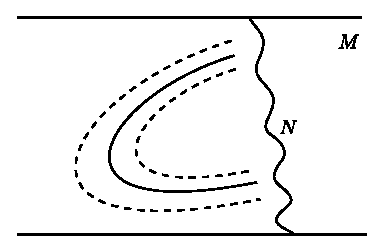
\includegraphics{vol46-fig/fig46-4.eps}
\end{figure}


If\pageoriginale $\varphi_i$(Int $D)\subset$ int $M$ delete from $M$
the tubular neighbourhood of $\varphi_i (D)$ (Refer to diagram $5''$).  

\begin{figure}[H]
\centering
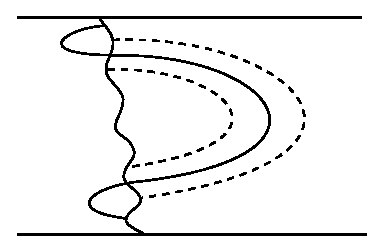
\includegraphics{vol46-fig/fig46-5.eps}
\end{figure}


The new manifold $M'$ with boundary $N'$ is still a 0-neighbourhood of
$\alpha$. Moreover, $\pi_1 N'$ is a quotient of $\pi_1 N$ and the
kernel of $\pi_1 N'  \to \pi_1 W$ is still (normally) generated by the
classes of $\varphi_j(S^1)$, $j = 1, \ldots, K$ with $j \neq i$ if $C =
bD^2$ for $\varphi_i$. But the $\varphi_j$ extend to $\varphi_j = D^2 \to M'$ with
$\varphi_j \varphi_j (D)^2 \cap N'$ consisting of one  less component curve
than the original intersection. After a finite number of such steps,
one reaches a 0-neighbourhood $M$, $bM = N$, such that $\pi_1 N\to
\pi_1 W$ is an isomorphism. By Lemma \ref{chap2:lem2.8}, $(M, N)$ is then a 
1-neighbourhood.  

\section[The Existence of Arbitrary small...]{The Existence of Arbitrary small $k.$ Neighbourhoods of
  ``$\infty$'' and ``$-\infty$'' for $2 \leq k \leq n - 2$}\label{chap2:sec3}%%% 3

\begin{definition}%defini 3.1
Let $k$ be an integer $\geq 2$. A $k$-neighbourhood of $\infty$ (respy
$-\infty$) in $W$ is a 1-neighbourhood $M$ of $\infty$
(respy $-\infty$) satisfying the following additional condition: 

Denoting\pageoriginale the universal covering of $M$ by $\tilde{M}$
with $p : \tilde{M} \to M$ the projection, let $\tilde{N} = p^{-1}
(N)$ where $N = bM$. The condition to be satisfied is : $H_i
(\tilde{M}, \tilde N) = 0$ for $i \leq k$.  
\end{definition}

\begin{remark*}
Since $\pi_1 (N)\to \pi_1(M)$ induced by the inclusion is an
isomorphism it follows that $p : \tilde{N} \to N$ is the universal
covering of $N$. 
\end{remark*}

\setcounter{prop}{1}
\begin{prop}\label{chap2:prop3.2}%proposi 3.2
There exist arbitrary small k-neighbourhoods of $\infty$
(respy `$-\infty$') for any integer $k$ such that $2 \leq k \leq n -
2$. 
\end{prop}

We prove this proposition for $k = 2$ first and then proceed by
induction on $k$. It will be clear from the proof why we are forced to
give a proof for $k = 2$ separately. 

\setcounter{lemma}{2}
\begin{lemma}\label{chap2:lem3.3}%lemma 3.3
If $M$ is a 0 (respy 1) neighbourhood of `$\infty$' then $M_\circ =
\overline{W - M}$ is a 0 (respy 1) neighbourhood of `$-\infty$'. 
\end{lemma}

\begin{proof}
Clearly the boundary of $M_\circ$ is the same as that of $M$. Thus $bM_\circ =
bM = N$ is compact and connected. If $m_1 < m_2$ are integers such
that $F^{-1} [m_1,\infty) \supset M \supset F^{-1} [m_2, \infty)$ then
    clearly $F^{-1} (-\infty, m_1] \subset M_\circ \subset F^{-1}
  (-\infty, m_2]$. Let $a, b$ be any two points in $M_\circ$. We will show
that there is an 
    arc in $M_\circ$ joining $a$ and $b$. Since $W$ is arcwise connected
    $\exists$ an arc $\sigma$ in $W$ with $\sigma (o) = a$ and $\sigma (1)
    = b$. If the arc $\sigma$ lies in $M_\circ$ there is nothing to
    prove. If not $\exists$ real numbers $t_\circ$ and $t_1$ such that
    $\tau(t) \in M_\circ$ $\forall$ $t \leq t_\circ$ and $\sigma (s) \in
    M_\circ$ $\forall$ $s \geq t_1$ and $\sigma (t_\circ) \in N$, $\sigma
    (t_1) \in N$. Choosing an arc in $N$ joining $\sigma (t_\circ)$
    and $\sigma (t_1)$ we see that $a$ and $b$ can be joined by means
    of an arc in $M_\circ$. Thus $M_\circ$ is a 0-neighbourhood of\pageoriginale
    `$-\infty$'. If $M$ is a 1-neighbourhood of $\infty$ then $\pi_1
    (bM) = \pi_1 (bM_\circ) = \pi_1 (N) \to \pi_1 (W)$ is an isomorphism
    and from Lemma \ref{chap2:lem2.8} it follows that $M_\circ$ is a 1-neighbourhood. 
\end{proof}

\begin{lemma}\label{chap2:lem3.4}%lemma 3.4
If $M$ is a 1-neighbourhood of $\infty$ in $W$, then $H_j (\tilde{M})$
is a finitely generated $\mathbb{Z} (J)$-module. 

For this we shall use assumption that $\mathbb{Z} (\pi)$ is a
noetherian ring. By an example of $J$.  Stallings the above lemma is
definitely false without this hypothesis. However, we really only need
that if $(M, N)$ is a $(k-1)$-neighbourhood, then $H_k (\tilde{M},
\tilde{N})$ is finitely generated. In the general case
($\mathbb{Z}(\pi)$ not necessarily noetherian) one proved that $(M, N)$
is dominated by a finite complex pair. It is then an exercise to
deduce from this the finite generation of $H_k (\tilde{M},
\tilde{N})$.	 
\end{lemma}

\begin{proof}
Let $N = bM$ and $M_\circ = \overline{W - M}$. By lemma
\ref{chap2:lem3.3}, $M_\circ$ is a 
1-neighbourhood of ``$ - \infty$''. If $W$ is the universal covering
of $W$ with $p : \tilde{W} \to W$ the projection there $\tilde{M} =
p^{-1} (M)$. $\tilde{M_\circ} = p^{-1}(M_\circ)$ and $\tilde{N} = p^{-1} =
p^{-1} (M \cap M_\circ) = \tilde{M} \cap \tilde{M}_\circ$ are respectively the
universal covering of $M$, $M_\circ$ and $N$. This is so because $\pi_1 (N)
\rightarrow \pi_1 (W)$, $\pi_1 (M) \rightarrow \pi_1 (W)$ and $\pi_1 (M_\circ)
\rightarrow \pi_1(W)$ induced by the respective inclusions are
isomorphisms. From the Mayer-Vietoris sequence 
$$
H_j (\tilde{N}) \rightarrow H_j (\tilde{M}_\circ) \oplus H_j (\tilde{M}) 
\rightarrow H_j (\tilde{W}) 
$$
which is sequence of $\mathbb{Z} \pi$-modules it will follow that $H_j
(\tilde{M})$ is finitely generated over $\mathbb{Z} (\pi)$ if we show that
$H_2 (\tilde{N})$ and $H_2(\tilde{W})$ are finitely generated over
$\mathbb{Z}(\pi)$. Since $N$ is smooth and compact,
choosing\pageoriginale a 
triangulation of $N$ we see that the chain groups of
$\tilde{N}$ with the lifted triangulation are finitely generated over
$\mathbb{Z} \pi$. From the fact that $\mathbb{Z} \pi$ is noetherian
again it follows that all the homology groups of $\tilde{N}$ are
finitely generated $\mathbb{Z}\pi$-modules. Also $W$ is of the
homotopy type of the finite polyhedron $X$ and the same argument as
above yields that all the homology groups of $W$ are	finitely
generated $\mathbb{Z} \pi$-modules. 
\end{proof}

\begin{lemma}\label{chap2:lem3.5} %lem 3.5
There exist arbitrary small 2- neighbourhoods of ``$\infty$''.
\end{lemma}

\begin{proof}
Let $M'$ with $bM' = N'$ be a 1-neighbourhood of $ \infty$ with $M'
\subset W - K$. By Lemma \ref{chap2:lem3.4}, $H_2 (M')$ is finitely generated over $
\mathbb{Z} (\pi)$. Let $ \alpha_1, \ldots , \alpha_r $ be a system of
generators over $\mathbb{Z} (\pi)$ for $H_2 (\tilde{M'}) = \pi_2
(\tilde{M'}) \sim \pi_2 (M')$. Choosing a small contractible open set
in Int $M'$ as the base point represent the elements $\alpha_i$ by
$C^\infty$ imbeddings $\varphi_i$: $S^2 \rightarrow$ Int $M'$, with
disjoint images and the base point of $S^2$ going into the chosen
contractible open set. For this to be possible we need that $\dim M'
\geq 5$ but by assumption $\dim M' = n+1 \geq 6$. Let $M$ be formed
from $M'$ as explained below: Choose closed tubular neighbourhoods
$T_i$ of $\varphi_i (S^2)$ in Int $M'$ with $T_i \cap T_j = \phi$
whenever $i \neq j$. Choose $C^\infty$ paths $\sigma_i$ from $N'$ to
$b T_i$ (the boundary of $T_i$) meeting $N'$ and $bT_i$ transversally
and at the end points only. These paths can be chosen to be mutually
disjoint, and tubular neighbourhoods $\Gamma_i$ of $\sigma_i$ can be
chosen to be mutually disjoint. Let $M = M' - \bigcup\limits^r_{i =
  1}$ Int $\cup T_i$ Int $\Gamma_i$. Then clearly $M$ is a
0-neighbourhood\pageoriginale of $\infty$. We claim that $M$ is a
2-neighbourhood of $\infty$. First 
of all, if $N = bM$ it is clear that $N = N' \# bT_1 \# \cdots
\# bT_r$ (connected sum). Also $bT_1$ is an $(n-2)$ sphere bundle
over $S^2$ with $n\geq 5$ and hence $\pi_1 (bT_i) = 1$. By Van Kampen
we see that $ \pi_1 (N) \simeq \pi_1 (N')$, under an isomorphism
making the following diagram commutative: 
\end{proof}
\[
\xymatrix@R=1.5cm{
\pi_1 (N) \ar[rr]^{\simeq} \ar[d]^{j_*} & & \pi_1 (N')\ar[d]^{j'_*}
\\
\pi_1(M) \ar[rr]^{\mu_*}\ar[dr]_{i_*} & & \pi_1 (M)
\ar[dl]^{i'_*}\\
& \pi_1 (W)& 
}
\]
\begin{center}
{\bf Diagram 6}
\end{center}

 Here the homomorphisms indicated by $i_*$, $j _*$, $i'_*$, $j'_*$ and
 $\mu_{*}$ are all induced by inclusions and the isomorphism $\pi_1
 (N) \to \pi_1 (N')$ is got from Van Kampen's theorem. It follows that
 $i_{*} o  j_{*}$ is an isomorphism since $i'_*$ and $j'_* $
 are. Lemma \ref{chap2:lem2.8}  now implies that $M$ is a 1-neighbourhood of
 $\infty$. 

\noindent
\textbf{Assertion:} $\pi_2 (N) \xrightarrow{j_*}\pi_2 (M)$ is an
epimorphism. 
 
 To prove this it suffices to show that $\pi_2 (N) \xrightarrow{\mu_*
\circ  j_*} \pi_2 (M') $ is an epimorphism and that $ \mu_{*}$: $\pi_2
 \to \pi_2(M')$  is an isomorphism.  Let\pageoriginale $\nu_i \in
 \pi_1$ $(So(n-1))$ be the element corresponding to the normal bundle of
 $\varphi_1 (S^2)$ in Int $M'$. As $S_*: \pi_1$ $(So (n-2))$ $\to
 \pi_1$ $(SO(n-1))$ is an isomorphism for $ n \geq 5$ we see that
 $\gamma_i$ can be written as $\gamma_i + \mathscr{O}^1$ is a trivial
 line bundle. Hence there exists a non zero cross-section for the
 associated sphere bundle. Using this cross-section we see that
 $\exists$ an element in $\pi_2(bT_i)$ which represents the element
 $\alpha_i \in \pi_2(M')$ under the inclusion $bT_i \to M'$. It
 now follows that $\pi_2 (N)\xrightarrow{\mu_* \circ j_*} \pi_2 (M')$ is an
 epimorhism. 
 
 This in particular gives: $\pi_2 (M) \xrightarrow{\mu_*}\pi_2(M')$ is
 an epimorphism. To complete the proof of the assertion we only to
 show that $\mu_*$ is a monomorphism. Let $x \in \pi_2 (M)$ be
 such that $\mu_*(x) = 0$ and let $ \theta : S^2 \to M$ be a
 $C^{\infty}$ imbedding representing $x$. The fact that $ \mu_* (x) = 0$
 implies that $ \exists$ a $C^{\infty}$ map $\varphi : D^3 \to M'$
 extending $\theta$. We can get $\varphi$ so as to be transverse regular
 on $\cup \varphi_i (S^2)$ (since $ \theta (S^2) \cap \varphi_i (S^2)
 = \phi)$. The condition $n + 1\geq 6 (n+1 = \dim M')$ implies that
 $\varphi(D^3)$ is then disjoint from $\cup \varphi_i (S^2)$. By a
 further deformation we can make $\varphi (D^3)$ go into $M$. 
 
 Now, $\pi _2(N) \xrightarrow {j _*}\pi _2(M)$ being an epimorphism we
 have $\pi_2 (\tilde{N}) \xrightarrow {j_*}\pi_2 (\tilde{M})$ also an
 epimorphism and hence $\pi_2 (\tilde{M}, \tilde{N}) = 0$. The simply
 connectedness of $\tilde{M}$ and $\tilde {N}$ now yields by the
 Relative Hurewicz Theorem  $H_2 (\tilde{M}, \tilde{N}) = \pi_2
 (\tilde{M}, \tilde{N}) = 0$. This completes the proof that $M$ is a
 2-neighbourhood. 
 
 We\pageoriginale now proceed to the proof of proposition \ref{chap2:prop3.2} for an
 arbitrary $k$ satisfying $3 \leq k \leq n-2$. Assume by induction
 that arbitrary small $(k-1)$ neighbourhoods of $\infty$ exist.  

 \begin{lemma}\label{chap2:lem3.6}%lemma 3.6
Suppose $M$ is any $(k-1)$-neighbourhood of $\infty$. Let $N = bM$. Then
\begin{enumerate}[(1)]
\item $H_k (\tilde {M}\tilde {N})$ \text{is a finitely
  generated} $\mathbb{Z} (\pi)$-module. 

\item $\exists$ another $(k-1)$-neighbourhood $M_1$ of $\infty$ with
  $M_1 \subset M$ satisfying the following additional condition: 
\end{enumerate}

The homomorphism $H_k (\tilde{U}, \tilde{N}) \to H_k (\tilde
{M}. \tilde {N})$ induced by the inclusion $(\tilde{U}, \tilde {N})
\subset (\tilde {M}, \tilde{N})$ is an epimorphism, where $U =
\overline{M - M_1}$ and $\tilde{U}$ is the inverse image of $U$ by the
covering map $p$: $\tilde M \to M$. 
 \end{lemma} 

\medskip
\noindent{\textbf{Proof of (1).}}
By Lemma 3.4 we have $H_j (\tilde{M})$ finitely generated over
$\mathbb{Z}(\pi)$ for every $j$. Also since $N$ is compact $H_j
(\tilde{N})$ is finitely generated over $\mathbb{Z} (\pi)$. The
exactness of $H_k (\tilde {M})\to H_k (\tilde{M},\tilde{N})\to
H_{k-1}(\tilde{N})$ together with Noetherian nature of
$\mathbb{Z}(\pi)$ now yield the finite generation of $H_k (\tilde{M},
\tilde{N})$ over $\mathbb{Z}(\pi)$. 


\medskip
\noindent{\textbf{Proof of (2).}}
Let $C_1, \ldots, C_\lambda$ be a finite set of generators for $H_k
(\tilde{M}, \tilde{N})$. There exists a compact set $\tilde{K}_1$ in $
\tilde{M}$ such that $\exists$ integral singular cycles representing
$C_1, \ldots, C_\lambda$ with their supports contained in
$\tilde{K}_1$. Let $K_1 = p(\tilde{K}_{1})$. By the inductive
assumption regarding existence of arbitrary small
$(k-1)$-neighbourhoods of $\infty$ we can find a $(k-1)$-neighbourhood
$M_1$ of $ \infty$ with $M_1 \subset W-K_1$ and $M_1 \subset M$. Then
clearly $ U = \overline{M-M_1}$ satisfies the condition $U \supset
K_1$  and thus the chosen cycles representing $C_1, \ldots,
C_{\lambda}$ are cycles of $(\tilde{U} ,\tilde{N})$. Hence
$H_k(\tilde{U}, \tilde{N}) \to H_k(\tilde{M},
\tilde{N})$\pageoriginale is onto.  

\begin{alphremark}\label{chap2:alphremA}%%% A
For the pair $(\tilde{U}, \tilde{N})$ we have $H_i 
(\tilde{U}, \tilde{N}) = 0$ for $i < k - 1$.  
 \end{alphremark} 

\begin{proof}
Let $N_1 = bM_1$. We have $H_i (\tilde{M}, \tilde{U})
\underset{\simeq}{ \longleftrightarrow}H _i (\tilde {M_i},
\tilde{N}_i)$ by excision. Now from the homology exact sequence of the
triple $(M, U, N)$ written below: 
{\fontsize{8}{10}\selectfont
\[
\xymatrix{
\ldots \ar[r] & H_{i+1} (\tilde{M}, \tilde{U}) \ar[r] & H_i(\tilde{U},
\tilde{N}) \ar[r] & H_i (\tilde{M}, \tilde{N}) \ar[r] & H_i
(\tilde{M}, \tilde{U}) \ar[r] & \ldots\\
& H_{i+1} (M_1, N_1) \ar[u]^{\approx}_{\rm excision} & & &
H_i(\tilde{M}_1, \tilde{N}_1) \ar[u]^{\approx}_{\rm excision}
}
\]}\relax 
 and the fact that $M_i$ is a $(k-1)$-neighbourhood of $\infty$ we see
 that $H_i (\tilde{U},\break \tilde{N}) \to H_i(\tilde{M}, \tilde{N})$ for $
 i < k-1$. Since $M$ itself is a $(k-1)$-neighbourhood we have
 $H_i(\tilde {U}, \tilde{N}) = 0$ for $i < k-1$. 
\end{proof}

\begin{alphremark}\label{chap2:alphremB}%%% B
 The homomorphisms $\pi_1 (N) \to \pi _1 (U)$ and $\pi_1
(N_1) \to \pi_1 (U)$ induced by the inclusions are isomorphisms. 
 \end{alphremark} 
 
 The proof of this is similar to the proof of Lemma \ref{chap2:lem2.8}
 and hence is omitted. 
 
 For completing the proof the proposition \ref{chap2:prop3.2} we need the following
 two propositions which we state without proof. 

\setcounter{prop}{6}
 \begin{prop}\label{chap2:prop3.7}%proposi 3.7
Suppose $U$ is a compact orientable $C^\infty$ manifold of dimension
$n+1$ with $n\geq 5$ and suppose $bU = N \cup N_1$ a disjoint union of
two open and closed, connected submanifolds of $bU$. If the
homomorphisms $\pi_1(N) \to \pi_1(U)$ and $\pi_1 (N_1) \to \pi_1(U)$
induced by the inclusions are isomorphisms and if $H_i (\tilde{U},
\tilde{N}) = 0$ for $i \leq k - 2 < n-2$ then\pageoriginale $(U, N)$
has a handle decomposition with handles of type $k-1$, $k,\ldots,
n-1$.  
 \end{prop} 
 
 \textit{In other words U has a presentation of the form}
 $$
 U = I \times N + \varphi _{1}^{k-1} + \cdots +
 \varphi^{k-1}_{\alpha_{k-1}} + \varphi^{k}_1+
 \varphi^{k}_{\alpha_{k}}+ \cdots +  \chi^{n-1}_1 + \cdots +
 \chi^{n-1}_{\alpha _{n-1}}. 
 $$
 
 The proof is essentially given in \cite{c2:key5}, Lemma 1.

 \begin{prop}\label{chap2:prop3.8}%proposi 3.8
Let $X$ and $Y$ be closed $C^ \infty$  submanifolds of a $C^ \infty$
manifold $N$, where $\dim X+ \dim Y= \dim N>4$, and $ 2< \dim Y \leq
\dim N-2$. Suppose that $\pi_1(N-Y) \to \pi_1 N $ induced by the
inclusion is an isomorphism. (This is a restriction only if $\dim Y=
\dim  N-2 $). Suppose that $X$ and $Y$ can be lifted to closed
submanifolds $\tilde{X}$ and $\tilde{Y}$ of $\tilde{N}$, the universal
covering of $N$, and that 
$$
\tilde X_i. \tau \tilde{Y}_j = 0
$$
(where denotes the homology intersection number) for all $\tau
\in \pi$ and all connected components $\tilde{X}_i$,
$\tilde{Y}_j$ of $\tilde{X}$ and $\tilde{Y}$. Then $X$ is isotopic in
$N$ to a submanifold $X_1$ such that $X_1 \cap Y = \phi$, or
equivalently $Y$ is isotopic in $N$ to a submanifold $Y_1$ such that
$X \cap Y_1 = \phi$. 
 \end{prop}

This proposition is essentially due to Whitney.

As remarked already proposition \ref{chap2:prop3.2} is proved by induction on $k$ for
$k$ in the range $3 \leq k \leq n-2$. Assume arbitrary small
$(k-1)$-neighbourhoods of $\infty$ exist. Let $K$ be any compact
subset of $W$ and let $M$ be any $(k-1)$-neighbourhood of $\infty$
with $ M \subset W-K$. By Lemma \ref{chap2:lem3.6}\pageoriginale $\exists$ a
$(k-1)$-neighbourhood 
of $\infty$ say $M_1$ with $M_1 \subset M$ such that the homomorphism
$H_k (\tilde{U}, \tilde{N}) \to H_k (\tilde{M}, \tilde{N})$ induced by
inclusion is onto, where $U =\overline{M - M_1}$ and $ bM = N$, $bM_1
= N_1$. From Remark \ref{chap2:alphremA} following Lemma
\ref{chap2:lem3.6} we have $H_i 
(\tilde {U}, \tilde {N}) = 0$ for $i <  k-1$ and by Remark
\ref{chap2:alphremB} the homomorphisms $\pi_1(N) \to \pi_1(U)$, 
$\pi_1(N_1) \to \pi_1(U) $ induced by the respective inclusions are
isomorphisms. Hence by proposition \ref{chap2:prop3.7} we have a handle
decomposition for $(U, N)$ with handles of type $k - 1$, $k, \ldots,
n-1$. Let $U_\circ$ be the union of $I \times N$ together with handles of
type $k-1$ (Refer to diagram 7) and $N_\circ$ the right hand boundary of
$U_\circ$. Let $U_1 = \overline{U-U_\circ}$. 

\begin{figure}[H]
\centering
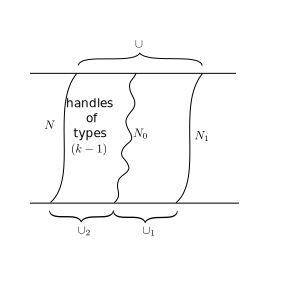
\includegraphics{vol46-fig/fig46-6.eps}
\end{figure}

\medskip
\noindent\textbf{Convention:} 
In future when we are in a situation of the form
$A \subset B$ or $(A, A') \subset (B, B') $ with $A$, $A'$, $B$, $B'$
topological spaces by the homomorphism $\pi_1 (A) \to \pi_1(B)$ or
$H_j (A) \to H_j (B) $ or $H_j(A, A')\to H_j(B, B')$ we mean the one
induced by the inclusion. When\pageoriginale $k>3$ we see from Van
Kampen theorem 
that $\pi_1(N) \to \pi_1 (U_\circ)$ is an isomorphism. When $k = 3$ we
first observe that the $2$-handles $\varphi^2_i$ are attached by means
of trivial maps to $1 \times N$. In fact $ \varphi^2_1 (S^1 \times 0)$
bounds a disk in $W$ and as $M$ is a 1-neighbourhood we have $\pi_1
(N) \to \pi_1 (W)$ an isomorphism. Now an application of Van Kampen
immediately yields $\pi_1 (N) \to \pi_1 (U_\circ)$ is an
isomorphism. Using the `dual' handle decomposition for $U_\circ$ and the
fact that $k \leq n-2$ we see that $\pi_1 (N_\circ) \to \pi_1 (U_\circ)$ is an
isomorphism, again by applying Van Kampen. To get $U_1$ we attach
handles of type $ k, \ldots, n-1$ to $U_\circ$. It follows that whenever
$k \geq 3$ the homomorphism $\pi_1 (N_\circ) \to \pi_1(U_1)$ is actually
an isomorphism. Now choose any $\alpha$ in $H_k (\tilde{M},
\tilde{N})$. By our choice of $M_1$ we have $H_k (\tilde{U},
\tilde{N}) \to H_k (\tilde{M}, \tilde{N})$ epimorphism. Choose any
$\beta \in H_k (\tilde{U}, \tilde{N})$ getting mapped onto
$\alpha$. By excision $H_k (\tilde{U}, \tilde{U_\circ}) \simeq H_k
(\tilde{U}_1, \tilde{N}_\circ)$ the isomorphism being a $\mathbb{Z}
(\pi)$-isomorphism since the maps induced by the various inclusions,
namely $N \to U_\circ$; $N_\circ \to U_\circ$ and $N_\circ \to U_1$ are isomorphisms
on $\pi_1$. Let $\gamma$ be the image of $\beta$ under the composition
of the maps 
$$ 
H_k (\tilde{U}, \tilde{N}) \xrightarrow{(\text{ inc } ln)_*} H_k 
(\tilde{U}, \tilde{U}_\circ)
\underset{\text{excision}}{\xleftarrow{\hspace{0.4cm}\simeq\hspace{0.4cm}}} 
 H_k  
(\tilde{U}_1, \tilde{N_\circ}). 
$$
Since $(U_1, N_\circ)$ has a handle decomposition with handles of type $k,
\ldots,\break n-1$ we that $H_i (\tilde{U}_1 \tilde{N}_\circ) = 0$ for $i \leq
k-1$ and by Relative Hurewicz theorem $ \pi_k (\tilde{U}_1,
\tilde{N}_\circ) \simeq  H_k (\tilde{U}_1, \tilde{N}_\circ)$. But $\pi_k
(\tilde{U}_1, \tilde{N}_\circ)  \simeq \pi_k (U_1, N_\circ)$. Thus $\pi_k (U_1,
N_\circ)\simeq H_k (\tilde{U}_1, \tilde{N}_\circ)$. 

\medskip
\noindent{\textbf{Claim:}}
 The element\pageoriginale $\gamma$ can be represented
by a $C^\infty$ imbedding $\varphi: (D^k, S^{k-1}) \to (U_1, N_\circ)$.   

Now, $\gamma$ is homologous to $\sum a_i D^k _i$ with $a_i \in
\mathbb{Z}(\pi)$ and $D^k _i$ the $k$-cell of the $i$-th hankle of
type $k$. $D^k _i$ is a differentiably imbedded $k$-cell in $U_1$ with
boundary $S_i^{ k-1}$ in $N_\circ$. Let $a_i= \sum\limits_{\sigma \in
  \pi} a_i^ \sigma \sigma$ with $ a_i^{(\sigma)}\in \mathbb{Z}$ and
$a_i^{(\sigma)}=0$ for almost all $\sigma$. We can assume that all the
$S_i^{k-1} D^{n-k+1}$ intersect a contractible open set in $N_\circ$ which
can be chosen as the ``base point'' for homotopy considerations. Let
$\ell_i= \sum\limits_{\sigma} | a_i^ \sigma |$. Let us take $\ell_i$
distinct points $x_1, \ldots,x_{\ell_i}$ in $D_i^{n-k+1}$. Form connected sum
of $D_i^k \times x_1, \ldots, D_i^k \times x_{\ell_i}$ along paths in
$N_\circ$ representing the $\sigma'$s for which $a_i^{(\sigma)} \neq
0$. This operation will give a $C^\infty$ imbedding $\theta_i$: $(D^k,
S^{k-1}) \to (U_1, N_\circ)$ representing $a_i D^k_i$. Forming connected
sum of the various $\theta_i (D^k)$ along trivial arcs in $N_\circ$ gives
a $C^\infty$ imbedding $\varphi: (D^k, S^{k-1}) \to (U_1, N_\circ)$
representing $\gamma$.  

Let $(D^k, S^{n-k+1}_j)$ be the boundaries of the right hand disks $D_j
^{n- k+2}$ corresponding to he handles of type $(k-1)$.  

\medskip
\noindent{\textbf{Claim:}}
 Let $\tilde{\varphi}(S^{k-1})$ and
$\tilde{S}^{n-k+1}_j$ be arbitrary lifts of $\varphi (S^{k-1})$ and
$S_j ^{n-k+1}$ to $N_\circ$. Then for any $\tau \in \pi$ the
homology intersection $\tilde{\varphi}(S^{k-1})$. $\tau
\tilde{S}^{n-k+1}_j$ in $\tilde{N}_\circ$ is zero. 
 
Actually $\tilde{\varphi} (S^{k-1})_{\dot{\tilde{N}_\circ}} \tau S_j^{n-k+1}$
is the same $\beta . \tau \{\tilde{S}_j^{n-k+1}$, this\pageoriginale later
intersection being the one associated to the pair $H_k (\tilde{U},
\tilde{N})$ and 
$H_{n-k+1} (\tilde{U})$. But $\left\{\tilde{S}^{n-k+1}_j\right \} = 0$
in $H_{n-k+1} (\tilde{U})$ since $\tilde{S}^{n-k+1}_j$ bounds a disk
in $\tilde{U}$.  

We now want to apply proposition \ref{chap2:prop3.8} to $\varphi (S^{k-1})=X$ and $Y=
US_j ^{n-k+1}$ which are submanifolds of $N_\circ$. To be able to apply
proposition \ref{chap2:prop3.8} we need to have $n-k+1 \leq n-2$ and $\pi_1 (N_\circ-Y)
\to \pi_1 (N_\circ)$ an isomorphism. The condition $n-k+1 \leq n-2$ gives
$k \geq 3$. This is precisely the reason why we had to prove the
existence of 2-neighbourhoods separately. We have already seen that
$\pi_1 (N) \to \pi_1 (U_\circ) $ and $\pi_1 (N_\circ) \to \pi_1 (U_\circ)$ are
isomorphisms. Since $\pi_1 (N_\circ) \to \pi_1 (W)$ is an isomorphism, it
follows that $\pi_1 (U_\circ) \to \pi_1 (W)$is an isomorphism and hence
$\pi_1 (N_\circ) \to \pi_1 (W)$ an isomorphism. Let $\varphi_j (D^{k-1}
\times D^{n-k+2})$ denote the handles of type $k-1$. Then the
inclusion $N_\circ -U \varphi _j(B^{k-1} \times S^{n-k+1}) \to N_\circ-
US_j^{n-k+1}$ is a homotopy equivalence, and $N - U \varphi_j (S^{k-2}
\times B^{n-k+2})=N_\circ -U\varphi_j (B^{k-1} \times
  S^{n-k+1})$. Consider the following commutative diagram:  
\[
\xymatrix{
\pi_1 (N - U \varphi_j (S^{k-2} \times B^{n-k+2})) \ar[r]\ar@{}[dd]|{||} & 
\pi_1 (N) \ar[dr] & \\
& &  \pi_1 (W)  \\
\pi_1 (N - U \varphi_j (B^{k-1} \times S^{n-k+1})) \ar[r] & \pi_1
(N_\circ - Y) \ar[r] &  \pi_1 (N_\circ) \ar[u] 
}
\]
\begin{center}
{\bf Diagram 8}
\end{center}

The map\pageoriginale
$$
\pi_1 (N-U_j \varphi_j (S^{k-2} \times B^{n-k+2})) \to \pi_1 N 
$$
is an isomorphism because it factors through $\pi_1 (N- U_j \ \varphi
_j (S^{k-2} \times\break B^{n-k+2})) \to \pi_1 (N-U_j \varphi_j (S^{k-2} \times
0)) \to \pi_1 N$, where the first map is induced by a homotopy
equivalence, and the second is also an isomorphism since codim
$S^{k-2}= n-k+2 \geq 3$. 

Thus proposition \ref{chap2:prop3.8} can be applied and it yields the following
conclusion. The imbedding $\varphi$ can be so chosen that
$\varphi(S^{k-1}) \cap Y= \phi$. It now follows from Morse theory that
$\varphi (S^{k-1})$ is diffeotopic in $U_\circ$ to an imbedding $\varphi'
: S^{k-1} \to N$. Actually one gets a $C^ \infty$ imbedding $\Phi$:
$S^{k-1}\times I \to U_\circ$ extending $\varphi$ i.e $\Phi | S^{k-1} \times
0= \varphi$ and satisfying $\Phi (S^{k-1} \times I) \subset N$. Taking
the diffeotopy together with the imbedding $\varphi$: $(D^k, S^{k-1})
\to (U_1, N_\circ)$ we get an imbedding $\varphi$: $(D^k, S^{k-1}) \to (U,
N)$. (See diagram 9). 

\begin{figure}[H]
\centering
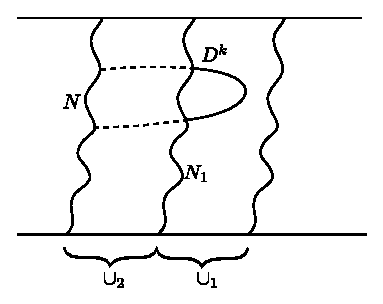
\includegraphics{vol46-fig/fig46-7.eps}
\end{figure}

The homology class in $H_k (\tilde{U},
\tilde{N})$ represented by $\varphi$ clearly gets ma\-pped into the
homology class $\gamma$ represented by $\varphi$ in $H_k (\tilde{U_1},
\tilde{N}_\circ)$ under the composition $H_k (\tilde{U}, \tilde{N}) \to H_k
(\tilde{U}, \tilde{U}_\circ) \xleftarrow[ \simeq]{\text{excision}} H_k
(\tilde{U_1}, \tilde{N}_\circ)$. From the exact sequence of the triple
$\tilde{U}$, $\tilde{U}_\circ$, $\tilde{N}$ we have 
$$
H_k (\tilde{U}_\circ, \tilde{N}) \to H_k (\tilde{U}, \tilde{N})\to H_k
(\tilde{U}, \tilde{U}_\circ) \text{ exact }. 
$$
But\pageoriginale $H_k (\tilde{U}_\circ, \tilde{N}) = 0$ since the handle
decomposition 
of $( U_\circ, N)$ we have, consists only of handles of type $ (k-1)
$. Thus $H_k (\tilde{U}, \tilde{N}) \to H_k (\tilde{U}, \tilde{U}_\circ)$
is a monomorphism and hence $\beta$ is the only element of $H_k
(\tilde{U}, \tilde{N})$ getting mapped into $\gamma$. It follows that
the class in $H_k (\tilde{U}, \tilde{N})$ represented by $\varphi$:
$(D^k, S^{k-1}) \to (U,N)$ is $\beta$. 

Let $A$ be the union of a tubular neighbourhood of $\varphi (D^k)$ in $M$
together with a tubular neighbourhood of $N$ in $M$. Define $M'$ to be
$\overline{M-A}$. Let $N'=bM'$. 

\noindent
\textbf{Claim:}\textit{$M'$ is a $(k-1)$-neighbourhood of $\infty$
  with $H_k(\tilde{M'}, \tilde{N'})\simeq H_k (\tilde{M},\break \tilde{N})/
  (\alpha)$ as a $\mathbb{Z}(\pi)$-module.} Here $(\alpha)$ denotes
the $\mathbb{Z}(\pi)$-submodule of $H_k (\tilde{M}, \tilde{N})$
generated by $\alpha$. 

Clearly $M'$ is a 0-neighbourhood of $\infty$ and from Van Kampen's
theorem we see that for $k$ satisfying $3 \leq k \leq n-2$  $\pi_1 (N')
\to \pi_1 (N)$ and $\pi_1 (M') \simeq \pi_1 (M)$ where the latter
isomorphism is induced by the inclusion. Also the isomorphism $\pi_1
(N') \to \pi_1 (N)$ makes the diagram 
\[
\xymatrix@R=1.5cm@C=1.5cm{
\pi_1 (N') \ar[r]^{\simeq}\ar[d]^{\rm(incln)_*} & \pi_1 (N)
\ar[d]^{\rm(incln)_*}_{\approx}\\
\pi_1 (M') \ar[r]^{\approx}_{\rm (incln)_*} & \pi_1 (M)
}
\]
commutative and hence $\pi_1 (N') \to \pi_1 (M')$ is an
isomorphism. It follows tht $M'$ is a 1-neighbourhood of $\infty$
. From the homology sequence of the triple $(\tilde{M}, \tilde{A},
\tilde{N})$ where $\tilde{A}= p^{-1}(A)$ with $p: \tilde{M}\to M$
the\pageoriginale covering map, we have the following diagram with the
horizontal row exact.  
\[
\xymatrix@R=1.5cm{
H_{i+1} (\tilde{M}, \tilde{A}) \ar[r] & H_i (\tilde{A}, \tilde{N})
\ar[r] & H_i(\tilde{M}, \tilde{N})  \ar[r] & H_i (\tilde{M},
\tilde{A}) \ar[r] & \\
H_{i+1} (\tilde{M}', \tilde{N}') \ar[u]_{\approx \text{ excision}} &
& & H_i (\tilde{M}', \tilde{N}')\ar[u]_{\rm excison}^{\approx} & 
}
\]
\begin{center}
{\bf Diagram 10}
\end{center}

Now, $H_i (\tilde{A}, \tilde{N}) = 0$ for $i \neq k$ and $H_k
(\tilde{A}, \tilde{N})=\mathbb{Z}(\pi)$ and the map $ H_i (\tilde{A},
\tilde{N}) \to H_i (\tilde{M}, \tilde{N})$ carries 1 of $\mathbb{Z}
(\pi)$ into $\alpha$. It follows that $H_i (\tilde{M'},\break \tilde{N'}) =
0$ for $i \leq k-1$ and that $H_k (\tilde{M'}, \tilde{N'})\simeq H_k
(\tilde{M}, \tilde{N})/ (\alpha)$. 

By Lemma~\ref{chap2:lem3.6} we have $H_k(\tilde{M}, \tilde{N})$ finitely generated
over $\mathbb{Z} (\pi)$.\break Choose a finite system of generators
$\alpha_1, \ldots, \alpha_r$ and apply the above procedure to $\alpha
= \alpha_1$. Then we get a $(k-1)$- neighbourhood $M'$ such that $H_k
(\tilde{M'}, \tilde{N'})$ is generated by the images of $\alpha_2,
\ldots, \alpha_r$ under the isomorphism $H_2 (\tilde{M'}, \tilde{N'})
\simeq H_2 (M, N)/ (\alpha_1)$. By interating this procedure a finite
number of times we finally arrive at a $k$-neighbourhood $M''$ of
$\infty$. Clearly $M'' \subset M \subset W-K$. This completes the
proof of Proposition \ref{chap2:prop3.2}. 

\section[The existence of arbitrary small...]{The existence of arbitrary small $(n-1)$- neighbourhoods of
  ``$\infty$''} \label{chap2:sec4}%%% 4

So far we have not used the hypothesis $\tilde{K}_\circ (\mathbb{Z} (\pi)) 
= 0$ any where. It is in the construction of arbitrary small
$(n-1)$-neighbourhoods of $\infty$ that we use this hypothesis. 

\begin{lemma}\label{chap2:lem4.1}% lemma 4.1 
 Let\pageoriginale $M$ be any $(n-2)$-neighbourhood of $\infty$ and
 let $N=   bM$. Then the homology. $H_*(\tilde{M}, \tilde{N})$ is the
 homology of a $\mathbb{Z}(\pi)$-chain complex of the form  
$$
0 \to \tilde{C}_{n-1} \xrightarrow{d} \tilde{C}_{n-2}\to 0 
$$
where $\tilde{C}_{n-1}$ and $\tilde{C}_{n-2}$ are free but not
necessarily finitely generated $\mathbb{Z}(\pi)$-modules. 
\end{lemma}

\begin{proof}
Pick a sequence of $(n-2)$-neighbourhoods
$$
M=M_\circ \supset M_1 \supset .. M_r \supset M_{r+1}\ldots.
$$
such that $\bigcup\limits_{r \geq 1} U_r = M$ where $U_r=
\overline{M_{r-1}-M_r}$. 
\end{proof}

We know that $\exists$ Morse functions $\lambda_r: U_r \to [r-1, r]$
with critical points of index $(n-2)$ and $(n-1)$ only, having the
components of $bU_r$ for level manifolds $\lambda^{-1}_{r}(r-1)$ and
$\lambda^{-1}_{r}(r)$ of $\lambda_r$. Thus $U_1$ is homotopically
equivalent to a space of the form $N \underset{\{f_i\}}{U} \underset{i \in
    I_1}{e_i^{n-2}} \underset{\{g_j\}}{U} \underset{j \in J_1}{e^{n-1}_j}
$ means of attaching a finite number of $(n-2)$ cells and
then a finite number of $(n-1)$ cells, under a homotopy equivalence
which is the identity on $N$. Choose a triangulation $L$ of $N$. By
the cellular approximation theorem to each of the characteristic maps
$f_i$ corresponds a homotopic cellular map $f'_i$: $S^{n-3} \to
L^{n-3} \subset L$. Thus $N \underset{\{f_i\}}{U}_{i \in I_1} e_i
^{n-2}$ is homotopy equivalent to the $CW$-complex $F= N
\underset{\{f'_i\}}{U} \underset{i \in I_1}{e_i ^{n-2}}$ under an
equivalence $\theta$ which is identity on $N$. 
Replacing\pageoriginale the maps $\theta \circ g_j$ by cellular maps
$g'_j: S^{n-2}\to F$ we get a $CW$-complex $K_1 = F
\underset{\{g'_j\}}{U}_{j \in j_1} e_j^{n-1}$ and a homotopy
equivalence $h_1:U_1 \to K_1$ which is identity on $N$. Also $K_1$
contains $L$ as a subcomplex. Using the Morse function $\lambda_2$ we
see that $U_1 \cup U_2$ is of the homotopy type of a space of the form
$U_1 \underset{\{f_i\}}{U}_{i \in I_2} e_i^{n-2} 
\underset{\{g_j\}}{U}_{j \in I_2} e_j^{n-1}$ under an
equivalence which is identity on $U_1$. Taking cellular approximations
$f'_i$ to $h_1 \circ f_i$ and attaching $n-2$ cells by means of $f'_i$ to
$K_1$ we get a $CW$-complex $F_2$ and a homotopy equivalence $U_1
\underset{\{f_i\}}{U}_{i \in I_2} e_i ^{n-2} \xrightarrow{\theta_2}
 F_2= K_1 \underset{\{f_i\}}{U}_{i
  \in I_2} e_i ^{n-2}$ extending $h_1$. Taking cellular
approximations $g'_j$ to $\theta_2 \circ g_j$ and attaching $(n-1)$ cells
to $F_2$ by means of the maps $g'_j$ we get a $CW$-complex $K_2$
containing $K_1$ as a subcomplex and a homotopy equivalence $h_2$:
$U_1 \cup U_2 \to K_2$ extending $h_1$. Proceeding thus we construct a
sequence of $CW$-complexes $L \subset K_1 \subset K_2 \subset K_3
\ldots$ and homotopy equivalences $\underset{1}{h_r} : \underset{j}{U}
      \underset{r}{U_j} \to K_r$ such that $h_r$ is an extension of
      $h_{r-1}$ and $h_1 = Id$ 
on $N = L$. Let $K = \underset{r}{U}\underset{1}{K_r}$ provided with the ``union
topology'' i.e. to say a set in $K$ is closed if and only if its
intersection with each $K_r$ is closed in $K_r$. Then $h$: $M \to K$
defined by $h | U_1 \ldots U_r=h_r$ is seen to be a homotopy
equivalence, because fo J.H.C. Whitchead's theorem. In
fact\pageoriginale it is easy 
to see that $h$ induces isomorphisms of homotopy groups and
Whitehead's theorem asserts that a map of $CW$-complexes inducing
isomorphisms of homotopy groups is a homotopy equivalence. Since the
cells of $K$ that are not in $L$ are either of dimension $n-2$ or of
dimension $n-1$, we have proved Lemma \ref{chap2:lem4.1}.  

\setcounter{coro}{1}
\begin{coro}%corollary 4.2
$H_{n-1} (\tilde{M}, \tilde{N})$ is a finitely generated
  projective $\mathbb{Z}(\pi)$ - module. 
\end{coro}

The proof for the finite generation of $H_{n-1} (\tilde{M},
\tilde{N})$ over $\mathbb{Z}(\pi)$ is the same as that of
(1) of Lemma \ref{chap2:lem3.6}. Since $H_{n-1} (\tilde{M}, \tilde{N}) =
0$ for $i \leq n-2$ we see that $d:$ $\tilde{C}_{n-1} \to
\tilde{C}_{n-2}$ has to be onto. The free nature of $C_{n-2}$ implies
$\tilde{C}_{n-1} \Ker d \oplus \tilde{C}_{n-2}$. Now
$H_{n-1}(\tilde{M}, \tilde{N}) \simeq \Ker d$ is a direct summand of
the free module $\tilde{C}_{n-1}$ hence projective.  

For any integer $e \geq 0$ let $\sum \limits_e \mathbb{Z}(\pi)$ denote
the direct sum of $e$ copies of $\mathbb{Z}(\pi)$. Since $\tilde{K}_\circ
(\mathbb{Z}(\pi))=0$ it follows that $\exists$ an integer $e \geq 0$
such that $H_{n-1}(\tilde{M}, \tilde{N}) \oplus \sum \limits_e
\mathbb{Z}(\pi)$ is a free $\mathbb{Z}$-module of finite rank. Let the
rank of $H_{n-1} (\tilde{M}, \tilde{N})+ \sum\limits_e
\mathbb{Z}(\pi)$ be $r$. 

\setcounter{lemma}{2}
\begin{lemma}\label{chap2:lem4.3}% lemma 4.3
Given any compact set $K$ of $W \exists$ an $(n-2)$ neighbourhood $M$
of $\infty$ with $M \subset W-K$ such that $H_{n-1}(\tilde{M},
\tilde{N})$ is a free $\mathbb{Z} (\pi)$-module of finite rank, where
$N = bM$. 
\end{lemma}

\begin{proof}
Choose any $(n-2)$-neighbourhood $M'$ of $\infty$ with $M' \subset
W-K$, and let $N'= bM'$. 
\end{proof}

By corollary 4.2, $H_{n-1}(M', N')$ is a finitely generated projective\break
$\mathbb{Z}(\pi)$- module and hence $\exists$ an integer $e \geq 0$
such that $H_{n-1}(\tilde{M'}, \tilde{N'})+\sum \limits_e
\mathbb{Z}(\pi)$\pageoriginale is free over $\mathbb{Z}(\pi)$ of
finite rank say 
$r$. We can find an $(n-2)$-neighbourhood $M''$ of $\infty$ with $M''
\subset M'$ and $H_{n-1}(\tilde{U}, \tilde{N}')\to H_{n-1}
(\tilde{M'},\break \tilde{N'})$ onto, where $U= \overline{M'-M''}$(see 2,
Lemma \ref{chap2:lem3.6}). By Proposition \ref{chap2:prop3.7},
$(U,N')$ has a handle decomposition 
consisting of handles of type $(n-2)$ and $(n-1)$ only. Without even
changing $M'$ we can introduce $e$ pairs of mutually cancelling
handles of type $(n-2)$ and $(n-1)$. Let $M$ be formed by removing
from $M'$ the union of the interiors of tubular neighbourhoods of the
$e$ newly introduced handles of type $n-2$ and a tubular neighbourhood
of $N'$, and let $N= bM$. 

\bigskip
\noindent\textbf{Claim:}
 $M$ is an $(n-2)$-neighbourhood of $\infty$ such that
$H_{n-1}(\tilde{M}, \tilde{N})$ is a free $\mathbb{Z}(\pi)$-module of
rank $r$. 

Let $A$ be the union of the closures of the tubular neighbourhoods
removed and let $\tilde{A} = p^{-1}(A)$. Using Van Kampen and the fact
that $n-2 \geq 3$ we see that $M$ is a 1-neighbourhood of
$\infty$. Also $H_i (\tilde{A},\tilde{N'}) = 0$ for $i \neq n-2$ and
$H_{n-2}(\tilde{A}, \tilde{N}')= \sum \limits_e \mathbb{Z}(\pi)$. From
the homology exact sequence of the triple $ (\tilde{M'}, \tilde{A},
\tilde{N'})$,  
{\fontsize{10}{12}\selectfont
\[
\xymatrix{
H_j (\tilde{A}, \tilde{N}')  \ar[r] & H_j (\tilde{M}', \tilde{N}')
\ar[r] & H_j (\tilde{M}', \tilde{A}) \ar[r] & H_{j-1} (\tilde{A},
\tilde{N}') \ar[r] & \ldots  \\
& & H_j (\tilde{M}, \tilde{N})\ar[u]_{\text{ a excision}} & & 
}
\]}\relax
we see that $H_i (\tilde{M}, \tilde{N}) = 0$ for $i \leq n-2$ and that
$H_{n-1} (\tilde{M}, \tilde{N})= H_{n-1} + \sum \limits_e \mathbb{Z}
(\pi)$. But by the choice of $e$, this is a\pageoriginale free
$\mathbb{Z}(\pi)$-module of rank $r$. This completes the proof of
Lemma \ref{chap2:lem4.3}. 

\setcounter{remark}{3}
\begin{remark}\label{chap2:rem4.4}% remark 4.4
If $M$ is any $(n-2)$-neighbourhood of $\infty$ and if $M_1$ is
another $(n-2)$-neighbourhood of $\infty$ with $M_1 \subset M$ and
$H_{n-1} (\tilde{U}, \tilde{N})\to H_{n-1} (\tilde{M}, \tilde{N})$
onto, (where U=$\overline{M-M_1}$) then $H_{n-1} (\tilde{U},
\tilde{N})\to H_{n-1} (\tilde{M}, \tilde{N})$ and $H_{n-1}
(\tilde{M_1}, \tilde{N}_1) = H_{n-2} (\tilde{U}, \tilde{N})$. 
\end{remark}

\begin{proof}
In the homology exact sequence 
of the triple $(\tilde{M}, \tilde{U}, \tilde{N})$ we have $H_n
(\tilde{M}_1, \tilde{N}_1) = 0$ by Lemma \ref{chap2:lem4.1}. By assumption
$H_{n-1}(\tilde{U}, \tilde{N}) \to H_{n-1}(\tilde{M}, \tilde{N})$ is
an epimorphism. It is now immediate that $H_{n-1}(\tilde{U},
\tilde{N}) \simeq H_{n-1}(\tilde{M}, \tilde{N})$ and that
$H_{n-1}(\tilde{M}_1, \tilde{N}_1)\simeq H_{n-2} (\tilde{U},
\tilde{N})$. 

Let $M$ be an $(n-2)$-neighbourhood of $\infty$ with
$H_{n-1}(\tilde{M}, \tilde{N})$ a free $\mathbb{Z}(\pi)$-module of
finite rank (say $r$). We can find a translate $M_1$ of $M$ by a Deck
transformation such that $M_1: M$ and $H_{n-1} (\tilde{U},
\tilde{N}) \to H_{n-1} (\tilde{M}, \tilde{N})$ onto, where $U=
\overline{M-M_1}$. We have to only choose the translate $M_1$ so as
not to intersect the compact set got as the projection by $p$ of the
union of supports of singular cycles (integral) representing a basis
for $H_{n-1}(\tilde{M}, \tilde{N})$ over $\mathbb{Z}(\pi)$ (See 2 of
Lemma \ref{chap2:lem3.6}). Corresponding to any handle decomposition of $(U, N)$ with
only handles of type $(n-2)$ and $n-1$ we get a chain complex $0 \to
\tilde{C}_{n-1}\overset{d}\to \tilde{C}_{n-2} \to 0$ whose homology
will precisely be $H_* (\tilde{U} \tilde{N})$. 

\begin{landscape}
\vbox to\textheight{\vfill%
\[
\xymatrix{
H_n (\tilde{M}, \tilde{U}) \ar[r]^\partial & H_{n-1} (\tilde{U},
\tilde{N}) \ar[r] & H_{n-1} (\tilde{M}, \tilde{N}) \ar[r] & H_{n-1}
(\tilde{M}, \tilde{U}) \ar[r] & H_{n-2} (\tilde{U}, \tilde{N}) \ar[r]
& 0 \\
H_n (\tilde{M}_1, \tilde{N}_1) \ar[u]_{\text{ a excision}}& & &
H_{n-1} (\tilde{M}_1, \tilde{N}_1) \ar[u]_{a}^{\rm excision} & & 
}
\]\vfill}
\end{landscape}
\end{proof}



For\pageoriginale the modules $\tilde{C}_{n-1}$, $\tilde{C}_{n-2}$ the
cells corresponding to handles of type $(n-1)$ and $(n-2)$
respectively form a basis over $\mathbb{Z}(\pi)$.   

\setcounter{prop}{4}
\begin{prop}\label{chap2:prop4.5}%%% 4.5
There exists a handle decomposition for $(U, N)$ with $2m$ handles of
type $(n-2)$ and $2m$ handles of type $(n-1)$ (where $m$ is a certain
integer $\geq r$) such that the boundary operator $C_{n-1}
\xrightarrow{d} C_{n-2}$ with reference to the basis given by the
handles has a matrix of the form $\left (\begin{smallmatrix} X &
  0\\ 0 &S^{-1} T \end{smallmatrix}\right)$, where $S$ and $T$ are $m
\times m$ invertible matrices over $\mathbb{Z}(\pi)$ and $X$ is the $m
\times m$ matrix $\left ( \begin{smallmatrix} 0& 0\\ 0&
  I_{m-r} \end{smallmatrix} \right)$. 
\end{prop}

\begin{proof}
By remark \ref{chap2:rem4.4} we have $H_{n-1}(\tilde{U}, \tilde{N})\simeq
H_{n-1}(\tilde{M}, \tilde{N})$ and $H_{n-2}(\tilde{U},\break
\tilde{N})\simeq H_{n-1}(\tilde{M_1}, \tilde{N_1})$. Since $M_1$ is a
translate of $M$ we have $H_{n-1}(\tilde{M}, \tilde{N})\simeq
H_{n-1}(\tilde{M_1}, \tilde{N_1})$ and by our choice of $M$,
$H_{n-1}(\tilde{M}, \tilde{N})$ is a free $\mathbb{Z}(\pi)$-module of
rank $r$. The pair $(U,N)$ has a handle decomposition with only handles
of type $n-2$ and $n-1$. Choose one such and let $0 \to
\tilde{B}_{n-1} \xrightarrow{d} \tilde{B}_{n-2} \to 0$ be the complex
corresponding to the chosen handle decomposition, giving the homology
of the pair $(\tilde{U}, \tilde{N})$. Here $\tilde{B}_{n-1}$ and
$\tilde{B}_{n-2}$ are free $\mathbb{Z}(\pi)$-modules of finite
rank. Since the homology of the complex $B$ is the same as $H_*
(\tilde{U}, \tilde{N})$ we get the following exact sequence. 
$$
0 \to Imd \to \tilde{B}_{n-2} \to H_{n-2} (\tilde{U}, \tilde{N})
\xrightarrow[{r}]{\simeq}\mathbb{Z}(\pi)\to 0. 
$$
It follows that $Imd$ is finitely generated and
$\mathbb{Z}(\pi)$-projective. Adding a finite number of pairs of
mutually cancelling handles if necessary we can assume that $imd$ is a
free $\mathbb{Z}(\pi)$-module. (Here we use the fact that $Imd$ is
stably free since $\tilde{B}_{n-2}$ is free of finite
rank).\pageoriginale Also we 
have the exact sequence $0 \to H_{n-1} (\tilde{U}, \tilde{N})\simeq
\sum \limits_r \mathbb{Z}(\pi) \to \tilde {B}_{n-1} \xrightarrow{d}
Imd \to 0$. If the rank of the free $\mathbb{Z}(\pi)$-module $Imd$ is
$k$ then it follows that both $\tilde{B}_{n-1}$ and $\tilde{B}_{n-2}$
have rank $m$ where $m= k+r$ and that $\exists$ bases $u_1, \ldots
u_m$ of $\tilde{B}_{n-1}$ and $v_1, \ldots v_m$ of $\tilde{B}_{n-2}$
satisfying $du_1=\cdots =du_r= 0$; $du_{r+1} = v_{r+1}, \ldots, du_m
= v_m$. Thus the matrix of $d$ with reference to the bases $u_1,
\ldots u_m$ and $v_1, \ldots, v_m$ of $\tilde{B}_{n-1}$ and
$\tilde{B}_{n-2}$ respectively is $X= \left( \begin{smallmatrix} 0&
  0\\ 0& I_{m-r} \end{smallmatrix}\right)$. Let $e_1^{n-1}, \ldots
e_m^{n-1}$ and $e_1^{n-2}, \ldots, e_m^{n-2}$ be the natural bases for
$\tilde{B}_{n-1}$ and $\tilde{B}_{n-2}$ given by the handles and let
the matrix of $d$ with reference to this natural pair of bases be
$A$. Now add $m$ pairs of mutually cancelling handles of types $n-2$
and $n-1$. With respect to the handle decomposition of $(U, N)$ thus
obtained the chain modules $\tilde{C}_{n-1}$ and $\tilde{C}_{n-2}$ are
both free $\mathbb{Z}(\pi)$-modules of rank $2m$ and the matrix of $d$
with reference to the natural pair of bases constituted by the handles
is $\left( \begin{smallmatrix} A& 0\\ 0 &
  I_m \end{smallmatrix}\right)$. If $e^{n-1}_{m+1}, \ldots ,
e^{n-1}_{2m}$ and $e^{n-2}_{m+1}, \ldots , e^{n-2}_{2m}$ are the
elements of $\tilde{C}_{n-1}$ and $\tilde{C}_{n-2}$ respectively,
corresponding to the newly attached $m$ pairs of mutually cancelling
handles then $u_1, \ldots u_m$; $e_{m+1}^{n-1}, \ldots, e_{2m}^{n-1}$
and $v_1, \ldots v_m$; $e_{m+1}^{n-2}, \ldots e_{2m}^{n-2}$ form bases
for $\tilde{C}_{n-1}$ and $\tilde{C}_{n-2}$ with reference to which
the matrix of $d$ is $\left( \begin{smallmatrix} X & 0\\ 0 &
  I_m \end{smallmatrix}\right)$. Now, there exist elements $S$, $T
GL(m, \mathbb{Z}(\pi))$ such that $X = S A T^{-1}$. The
matrices\pageoriginale 
$\left (\begin{smallmatrix} S & 0\\ 0 & S^{-1} \end{smallmatrix}
\right)$ and $\left( \begin{smallmatrix} T^{-1} & 0\\ 0 &
  T\end{smallmatrix} \right)$ are products of elementary matrices in
  $GL(2m, \mathbb{Z}(\pi))$, and we have 
$$ 
\begin{pmatrix}
S & 0 \\ 
0 & S^{-1}
\end{pmatrix}
\begin{pmatrix}
A & 0\\ 
0 & I \end{pmatrix}
\begin{pmatrix}
T^{-1} & 0\\ 
0 & T\end{pmatrix}
=\begin{pmatrix}
X, & 0\\ 
0 & S^{-1} T
\end{pmatrix}
$$
Thus to prove proposition \ref{chap2:prop4.5} it suffices to prove the following. 
\end{proof}

\setcounter{lemma}{5}
\begin{lemma}\label{chap2:lem4.6}% lemma 4.6
One can change the matrix $\left( \begin{smallmatrix}A & 0\\ 0 &
  I\end{smallmatrix}\right)$ of $d$ by left or right multiplication by
  elementary matrices by performing an isotopy of the attaching map of
  the handles. 
\end{lemma}

\begin{proof}
Let $U= I \times N+ \varphi_1^{n-2}+ \cdots + \varphi_{2m}^{n-2}+
\varphi_1^{n-1}+ ..+ \varphi_{2m}^{n-1}$ be the handle decomposition which
gives the matrix $\left( \begin{smallmatrix}A & 0\\ 0 &
  I \end{smallmatrix} \right)$ for $d$. For each $i$ such that $1 \leq
i \leq 2m$ let $Y_i$ be the right hand boundary of $I \times N+
\varphi_1^{n-2}+\cdots+ \varphi_{2m}^{n-2}+$ all the handles of type
$(n-1)$ except the $i$ th. First we prove the lemma for left
multiplication by elementary matrices. We actually show that by an
isotopy of $\varphi_i$ into $Y_i$ one can change $d e_i^{n-1}$ by any
$\sum \limits_{j \neq i} x_j d e_j^{n-1} $ with arbitrary $x_j
\in \mathbb{Z} (\pi)$. For this it suffices to prove the same
assertion for $x_j d e_j^{n-1}$ for a particular $j \neq i$ and $x_j
\epsilon \pm \pi$. Now $\varphi_j (S^{n-2} \times *)$ with $*$ any point
on $bD^2$, is isotopic to the trivial imbedding in $Y_i$ for $i \neq
j$, because $\varphi_j (S^{n-2}\times *)$ bounds a cell on the boundary
of the handle $\varphi_j$. Perform ``connected sum'' of $\varphi_i$ and
$\varphi_j$ along an arc representing $x_j$ and take it as the new
$\varphi'_j$. For proving the lemma for multiplication on the right by an
elementary\pageoriginale matrix we look at the dual handle
decomposition. Let $U= I 
\times N_1 + \varphi_1 ^{*2}+\cdots+ \varphi_{2m}^{*2}+
\varphi_1^{*3}+ \cdots+ \varphi_{2m}^{*3}$ be the dual handle
decomposition. Let $0 \to \tilde{C}_3 \xrightarrow{d^*} \tilde{C}_2
\to 0$ be the chain complex corresponding to this handle
decomposition. With respect to the canonical bases of $\tilde{C}_3$
and $\tilde{C}_2$ constituted by the handles of type 3 and 2
respectively, the matrix of $d^*$ is the same as $\pm
\left( \begin{smallmatrix} A^* & 0 \\ 0 & I_m \end{smallmatrix}
\right)$ where $A^*= (a^* _{ij})$ with $a^*_{ij}=
\bar{a}_{ji}\ldots$. Here $(a_{ij})$ is the matrix $A$ and for each $a
\in \mathbb{Z}(\pi)$, $\bar{a}$ is the element which corresponds
to $a$ under the map which carries any $x \in \pi$ into the dement $\pm
x^{-1}$. (The sign depending on whether $x$ preserves $ (+)$ or
reverses $ (-)$ an orientation of $\tilde{U}$\,). Choose listings of $3$
and $2$ cells for the dual decomposition $\tilde{\varepsilon}_1^3,
\ldots \tilde{\varepsilon}^3_{2m}$; $\tilde{\varepsilon}^2_1, \ldots,
\tilde{\varepsilon}^2_{2m}$ so as to satisfy
$\tilde{e}^{n-2}_i. \tilde{\varepsilon}_j^3= \delta_{ij}$;
$\tilde{e}^{n-1}_i. \tilde{\varepsilon}_j^2= \delta_{ij}$ and
$\tilde{e}_i^{n-1}$. $\sigma \tilde{\varepsilon}_j^2= \delta_{ij}
\delta_{\sigma, 1}$ for every $\sigma \in \pi$. Using the formula
$\tilde{\varepsilon}_k^3. d \tilde{e}_i^{n-1}=d^*
\tilde{\varepsilon}_k^3. \tilde{e}_i^{n-1}$ (up to a sign which depends
only on $n$ and not on $i$ and $k$) it is easy to see that the matrix
of $d^*$ with reference to the pair of bases constituted by
$\tilde{\varepsilon}_1^3, \ldots , \tilde{\varepsilon}^3_{2m}$ and
$\tilde{\varepsilon}_1^2,\ldots , \tilde{\varepsilon}^2_{2m}$ is
precisely $\left( \begin{smallmatrix} A^* & 0\\ 0 &
  I \end{smallmatrix} \right)$(up to sign). Now, by what we have
proved already, this handle decomposition of $(U, N_1)$ can be altered
so as to alter the matrix $\left ( \begin{smallmatrix} A^* & 0\\ 0 &
  I \end{smallmatrix}\right)$ be left multiplication\pageoriginale by
an elementary 
matrix. Now, taking the dual of the altered handle decomposition we
get a handle decomposition for $(U, N)$ which alters the matrix $\left
(\begin{smallmatrix} A & 0\\ 0 & I \end{smallmatrix}\right)$ be right
multiplication by an elementary matrix. This proves Lemma \ref{chap2:lem4.6}. 
\end{proof}

We choose a handle decomposition for $(U, N)$ of the type mentioned in
Proposition \ref{chap2:prop4.5}. Then the Kernel of $d$: $\tilde{C}_{n-1} \to
\tilde{C}_{n-2}$ is the free $\mathbb{Z}(\pi)$-module of rank $r$ with
the elements $\tilde{e}_1^{n-1}, \ldots, \tilde{e}_r^{n-1} $
corresponding to the first $r$ handles of type $(n-1)$. 

\medskip
\noindent{\textbf{Assertion.}}
\textit{ Any one of the elements $\tilde{e}_i^{n-1} (1
\leq i \leq r) $ can be represented by a $C^\infty$ imbedding
$\theta_i: (D^{n-1}, S^{n-2})\to (U, N)$.} 

In fact $de_i^{n-1} = 0$ implies that any lifting
$\tilde{\varphi}_i(S^{n-2} \times *)$ of $\varphi_i (S^{n-2}\times *)$ has
trivial homology intersection in $N_\circ$ with any lifting
$\tilde{\varphi}_j (* \times S^2)$ of any of the transverse 2-spheres of
the handles of type $n-2$. (Here $N_\circ$ is the right hand boundary of
$I \times N+ \sum \limits^{2m}_{j=1} \varphi_j^{n-2}$). Now use
Proposition \ref{chap2:prop3.8} with $X= \sum \limits^{2m}_{j=1} \varphi_j (* \times
S^2)$ and $Y= \sum \limits^{2m}_{i=1} \varphi_i (S^{n-2} \times *)$. The
condition $\pi(N_\circ -Y) \to \pi_1 N_\circ$ an isomorphism is satisfied
because of the following diagram (where as above $N_1$ is the right
boundary of $U$): 
\[
\xymatrix{
  \pi_1 (N_\circ - Y) \ar[r]^>>>>>>\simeq \ar[d] & \pi_1 (N_1 - U^{2m}_{i=1}
  \varphi^*_i (D^{n-1} \times S^1)) \ar@{}[r]|>>>>>>{\simeq} & \pi_1 N_1 \ar[d]^\simeq\\
\pi_1 N_\circ \ar[rr]_{\simeq} & & \pi_1 W
}
\]

The\pageoriginale ``upper'' horizontal isomorphisms are obvious. The
isomorphism  
$\pi_1 N_1 \to \pi_1 W$ follows from the fact that $(M_1, N_1)$ is a
1-neigh\-bourhood. The ``bottom'' horizontal map is also an isomorphism
because $\pi_1 N_\circ \to \pi_1 U_1$ is an isomorphism ($U_1 = I\times
N_\circ+$ (handles of type $n-1$).) $\pi_1 U_1 \to \pi_1 U$ is also an
isomorphism since $U=U_1+$ (handles of type 3), and $\pi_1 U \to \pi_1
W$ has been noted to be an isomorphism before. (Recall Lemma \ref{chap2:lem2.8}.)
Using proposition \ref{chap2:prop3.8} as before we see that we can find $C^\infty$
imbeddings $\theta_i: (D^{n-1}, S^{n-2}) \to (U, N)$ representing
$\tilde{e}_i^{n-1} \in H_{n-1}(\tilde{U}, \tilde{N})$. Let $B$
the union of tabular neighbourhoods of $\theta_i (D^{n-1})$ and $N$ in
$M$ and let $M' = \overline{M-B}$. By Van Kampen it is easy to see
that $\exists$ an isomorphism $\pi_1 (N)\to \pi_1 (N')$ where $N'=
bM'$ and that the inclusion $M' \to M$ induces an isomorphism $\pi_1
(M') \to \pi_1 (M)$. Also the isomorphism $\pi _1 (N)\to \pi_1 (N')$
makes the diagram. 
\[
\xymatrix{
\pi_1(N) \ar[r] \ar[dd]^\approx & \pi_1 (M) \ar[dr]^\simeq
\ar[dd]_\simeq & \\
&  & \pi_1 (W) \\
\pi_1 (N') \ar[r] & \pi_1 (M') \ar[ur]
}
\]
commutative. It follows that $M'$ is a 1-neighbourhood. Now from the
homology exact sequence of the triple $\tilde{M}, \tilde{B},
\tilde{N}$ it follows that $H_i (\tilde{M'},\break \tilde{N'}) = 0$ for $i
\leq n-2$ and $H_{n-1}(\tilde{ M' }, \tilde{N'}) \simeq H_{n-1}(\tilde{M},
\tilde{N})/ (e_1, \ldots, e_r)=0$. Thus starting from any $(n-2)$
neighbourhood $M$ of $\infty$ with $H_{n-1}(\tilde{M}, \tilde{N})$
free\pageoriginale of rank $r$ over $\mathbb{Z}(\pi)$ we have
constructed a $(n-1)$ neighbourhood $M'$ of $\infty$ with $M' \subset
M$.  

\setcounter{prop}{6}
\begin{prop}\label{chap2:prop4.7}% proposition 4.7
There exist arbitrary small $(n-1)$-neighbourhoods of $\infty$.
 \end{prop} 
 
 \section{Completion of the proof of siebenmann's theorem}\label{chap2:sec5}%% 5
 
 \begin{lemma}\label{chap2:lem5.1}% lemma 5.1
Suppose $M$ and $M_1$ are two $(n-1)$ neighbourhoods of $\infty$ with 
$M \supset M_1$ and $bM_1= \phi$. Then $U= \overline{M-M_1}$ is a
$h$-cobordism between $bM$ and $bM_1$. 
 \end{lemma} 
 
 \begin{proof}
Denote $bM$ and $bM_1$ by $N$ and $N_1$ respectively. Then as already
observed $\pi_1 (N) \to \pi_1 (U)$, $\pi_1 (N_1) \to \pi_1 (U)$ are
isomorphisms. (Remark \ref{chap2:alphremB} after Lemma
\ref{chap2:lem3.6}). Since $M$ and $M_1$ are 
$(n-1)$-neighbourhoods we have $H_i (\tilde{M}, \tilde{N}) = 0 = H_i
(\tilde{M}_1, \tilde{N}_1)$ for all $i$. In fact by Lemma \ref{chap2:lem4.1}, $H_*
(\tilde{M}, \tilde{N})$  or $H_* (\tilde{M}_1, \tilde{N}_1) $
is the homology of a complex of the form $C \to \tilde{B}_{n-1} \to
\tilde{B}_{n-2} \to 0$. Thus $H_i (\tilde{M}, \tilde{N}) = 0$ for
$i>n$ and by definition of an $(n-1)$-neighbourhood of $\infty$ we have
$H_i (M, N) = 0$ for $i \leq n-1$. From the homology exact sequence of
the triple $(\tilde{M}, \tilde{U}, \tilde{N})$ 
we see immediately that $H_j (\tilde{U}, \tilde{N}) = 0$ for every
$j$. Thus to prove Lemma \ref{chap2:lem5.1} it only remains to show that $H_i
(\tilde{U}, \tilde{N_1})=0$ for every $j$. 

\begin{landscape}
\vbox to\textheight{\vfill%
\[
\xymatrix{
H_i (\tilde{U}, \tilde{N}) \ar[r] & H_i (\tilde{M}, \tilde{N}) \ar[r]
& H_i (\tilde{M},\tilde{U}) \ar[r] & H_{i-1} (\tilde{U}, \tilde{N})
\ar[r] & H_{i-1} (\tilde{M}, \tilde{N}) \ar[r] & \ldots\\
& & H_i(\tilde{M}_1, \tilde{N}_1) \ar[u]^{\rm excision}_u & & & 
}
\]\vfill}
\end{landscape}
 \end{proof}
 
 For\pageoriginale the pair $(U, N)$ we have a handle decomposition
 with handles of 
 type $n-2$ and $n-1$ only. If $0 \to \tilde{C}_{n-1}
 \xrightarrow{d} \tilde{C}_{n-2} \to 0$ is the corresponding complex
 given the homology of $(\tilde{U}, \tilde{N})$, from the fact that
 $H_i (\tilde{U}, \tilde{N})=0$ $\forall i$ it follows that $d$ is an
 isomorphism. If we use the dual handle decomposition for $(U, N_1)$
 the homology $H_* (\tilde{U}, \tilde{N}_1)$ will be the homology of a
 complex of the form $0 \to \tilde{C}_3 \xrightarrow{d^*} \tilde{C}_2
 \to 0$. If $A=(a_{ij})$ is the matrix of $d$ with respect to the
 bases constituted by the handles of type $(n-2)$ and $(n-1)$, then as
 already seen the matrix of $d^*$ with respect to the bases
 constituted by the handles of type 3 and 2 in the dual decomposition
 is $A^*= (a^*_{ij})$ (up to sign) where $a^*_{ij}=
 \overline{a_{ji}}$. It follows that if $d$ is an isomorphism so is
 $d^*$. Hence $H_* (\tilde{U}, \tilde{N}_1)=0$. 

 \setcounter{prop}{1}
 \begin{prop}\label{chap2:prop5.2}% proposition 5.2
Let $M$ be any $(n-1)$-neighbourhood of $\infty$ in $W$. Then $M$ is
diffeomorphic to $N \times [0, \infty)$ where $N=bM$. 
 \end{prop} 
 
 The proof of this proposition uses the $S$-cobordism theorem of\break
 Barden-Mazur-Stallings \cite{c2:key5}, \cite{c2:key6} or \cite{c2:key8}. Let
 $U$ be a $h$-cobordism  between two compact, connected oriented
 $C^{\infty}$ manifolds $V^n$  and $V'^n$ of dimension $n \geq
 5$. Using the isomorphisms $\pi_1 (V) 
 \to \pi_1 (U)$ and $\pi_1 (V')\to \pi_1 (U)$ we identify all the
 three groups $\pi_1 (V)$, $\pi_1 (U)$ and $\pi_1 (V')$ and abstractly
 denote any one of them by $\pi$. Let $\tau (U, V) \in Wh (\pi)$
 denote the torsion of the pair $(U, V)$. We now state the
 $S$-cobordims theorem which actually consists of two parts. 
 
\bigskip
 \noindent\textbf{S-Cobordism Theorem:}\pageoriginale
\textit{{\em (1)} The inclusion of $V$ in $U$ cab be extended into a
 diffeormorphism of $V \times I$ onto $U$ if and only if $\tau (U,
 V)=0$. } 

\smallskip
\noindent
\textit{{\em (2)} Given a compact, connected $C^\infty$ manifold $V^n$
 of dimension $n \geq 5$ and any $\tau \in Wh (\pi)$ where $\pi=
 \pi_1 (V)$, there exists a $h$-cobordism $U$ between $V$ and a
 certain $V'$ such that $\tau (U, V)= \tau$.}
 

For more information about torsion and the Whitehead group $Wh(\pi)$
refer to \cite{c2:key1}, \cite{c2:key5} or \cite{c2:key13}. We list below some
known properties of torsion that we need for the proof of Proposition
\ref{chap2:prop5.2}.  
 
 The symbols $V$, $V'$, $V_1$, $V'_1$ etc. are used to denote
 connected, compact, $C^\infty$ manifolds. Let $U_1$ be a $h$-cobrdism
 between $V_1$ and $V'_1$, and $U_2$ a $h$-cobordism between $V_2$ and
 $V'_2$. Let $g: V_2 \to V'_1$ be a diffeomorphism of $V_2$ onto
 $V'_1$. Let $U=U_1 \, \underset{g}{.} \, U_{2}$ be the differential manifold
 got from the union of $U_1$ and $U_2$ by identifying $V_2$ with
 $V'_1$ by means of the diffeomorphism $g$. The groups $\pi_1 (V_1)$,
 $\pi_1 (U_1)$ and $\pi_1 (V'_1)$ are all identified as explained
 already and let $\pi_1$ denote any one of them. Let $\pi_2$ have a
 similar meaning with respect to $V_2, U_2$ and $V'_2$ (i.e. $\pi_2=
 \pi_1(V_2)$ etc.). The diffeomorphism $g$ induces an isomorphism $g*$:
 $\pi_2 \to \pi_1$. If $\tau_1 = \tau(U_1, V_1) \in Wh
 (\pi_1)$ and $\tau_2 = \tau (U_2, V_2) \in Wh (\pi_2)$ then
 $U=U_{1\dot{g}} U_2$ is a $h$-cobordism between $V_1$ and $V'_2$
 satisfying $\tau(U, V_1)= \tau_1 + g_* (\tau_2)$. In particular if
 $U_1$ is a $h$-cobordism between $V$ and $V'$ and if $U_2$ is a
 $h$-cobordism between $V'$ and a certain $V''$ such that $\tau (U',
 V') = - \tau (U, V)$ then $U_1$. $U_2$ is diffeomorphic\pageoriginale
 to $V \times 
 I$ whenever $\dim V(= \dim V') \geq 5$. If $U$ is a $h$-cobordism
 between $V$ and $V'$ with torsion $\tau (U,V)$, we can construct a
 $h$-cobordism $U^{-1}$ from $V'$ to some $V''$ with torsion $\tau
 (U^{-1}, V')=- \tau (U, V)$. (Use part (2) of the
 $S$-cobordism theorem). Then, pasting $U$ and $U^{-1}$ along $V'$ by
 the identity mapping, the $h$-cobordism $U U^{-1}$ form $V$ to $V''$
 has torsion $\tau (U, V)+ \tau (U^{-1}, V') = 0$. It follows by part
 (1) of the $S$-cobordism theorem that $U \cup U^{-1}$ is
 diffeomorphic to $V-I$ and in particular that $V$ and $V''$ are
 diffeomorphic. The formation of products of $h$-cobordisms satisfies
 the following associativity rule. Let $U_i(i= 1, 2, 3)$ be a
 $h$-cobordism between $V_i$ and $V'_i$ and let $g: V_2 \to V'_1; h:
 V_3 \to V'_2$ be diffeomorphisms. Then $\exists$ a diffeomorphism
$\alpha : (U_1 \underset{g}{\cdot} U_2) \underset{h}{\cdot} U_3 \to U_1
 \underset{g}{\cdot} (U_2 \underset{h}{\cdot} U_3)$
extending the identity map of $V_1$. Also if $U$ is a
 $h$-cobordism between $V$ and $V' \exists$ a diffeomorphism $\beta$:
 $ U \to U. V' \times I$ with $\beta|V= Id_V$ and $\beta (v')= (v', 1)$
 $\forall \, v' \in  V'$. (This is a consequence of the fact that $V'$ is
 differentiably collared in $U$). For the proof of Proposition \ref{chap2:prop5.2} we
 need the following Lemma on infinite products of $h$-cobordisms. 
 
\setcounter{lemma}{2}
 \begin{lemma}\label{chap2:lem5.3} %lemma 5.3
 For every integer $k \geq 1$ let $U_k$ be a $h$-cobordism between
 $V_k$ and $V'_k$ and let $V'_k= V_{k+1}$. If dim $V_1 \geq 5$ then
 the infinite product $U_1. U_2. U_3. \ldots$ is diffeomorphic to $V_1
 \times [0, \infty)$. 
\end{lemma} 

\begin{proof}
As\pageoriginale observed already $\exists$ diffeomorphisms $\beta_k$:
$U_k \to 
U_K. V'_k I$ with $\beta_k | V_k=Id_{V_k}$ and $\beta_k (v') = (v',
1)$ $\forall \,  v' \subset V'_k$. Hence the infinite product
$U_1. U_2. U_3. \ldots$. is also diffeomorphic to the infinite
product $U_1. V'_1 \times I$. $U_2$. $V'_2 \times I$. $U_3$. $V'_3
\times I. \ldots$. For every integer $k \geq 1$ the product
$U_k^{-1}. U_{k-1}^{-1}. \ldots U_1^{-1}$. $U_1. \ldots U_k$ is a
$h$-cobordism with torsion zero. Therefore $\exists$ a
diffeomorphism. $\theta_k$: $V'_k \times I \to U^{-1}_k \ldots. U_1
^{-1}$. $U_1. \ldots U_k$ satisfying $\theta_k (v', 0) = v'$ of the
left hand boundary of $U^{-1}_k. \ldots . U_1 ^{-1}$. $U_1 \ldots
U_k$. The map $v' \to \theta_k (v', 1)$ is a diffeomorphism $g_k$ of
$V'_k$ onto the right hand boundary of $U_k^{-1}. \ldots
U_1^{-1}$. $U_1. \ldots U_k$. Now it is clear that the product
$U_1$. $V'_1 \times I$. $U_2$. $V'_2 \times I$. $U_3$. $V'_3 \times
I$. $U_4 . \ldots. $ is diffeomorphic to the product  
{\fontsize{10}{12}\selectfont
$$
U_1. (U_1^{-1}. U_1) \underset{g_1}{\cdot}  U_2. (U_2^{-1}. U_1
^{-1}. U_1. U_2) \underset{g_2}{\cdot}  U_3. (U_3^{-1}. U_2^{-1}. U_1
^{-1}. U_1. U_2. U_3) \underset{g_3}{\cdot} U_4 \ldots. 
$$} 

Also it is clear that the diffeomorphism $g_k$: $V'_k \to V'_k$ is
homotopic to the identity map of $V'_k$ and hence $g_{k*}$: $\pi \to
\pi$ is the identity map. Since product formation of $h$-cobordisms is
an associative operation we have  
$$
U_1. (U_1^{-1}. U_1) \underset{g_1}{\cdot} U_2. (U_2 ^{-1}. U_1
^{-1}. U_1. U_2) \underset{g_2}{\cdot} \ldots .\text{ diffeomorphic to } 
$$ 
$$
U_1. U_1^{-1}. (U_1 \underset{g_1}{\cdot} U_2. U_2 ^{-1}. U_1 ^{-1}). (U_1. U_2
\underset{g_2}{\cdot} U_3. U_3^{-1}. U_2 ^{-1}. U_1^{-1}). \ldots . 
$$
Denoting\pageoriginale the products $U_1. \ldots U_k$; $U_1 \ldots U_k
\underset{g_k}{\cdot}  U_{k+1}. U_{k+1}^{-1} \ldots U_1^{-1}$ and
$U_{k+1}$. $U_{k+1}^{-1}$. $U_k^{-1}. \ldots U_1 ^{-1}$ by $A_k$;
$B_k$ and $C_k$ respectively we have $\tau (B_k,\break V_1) = \tau (A_k,
V_1)+(g_k)_*$ $(\tau (C_k, V_{k+1}))= \tau (A_k, V_1) + \tau (C_k,
V_{k+1})$ since $g_{k*}$ is the identity map. But $\tau (A_k, V_1)+
\tau (C_k, V_{k+1}) = 0$. Hence the inclusion of $V_1$ into $B_k$ as
the left hand boundary extends to a diffeomorphism of $V_1 \times I$
onto $B$. It follows that the product 
$$
(U_1. U_1 ^{-1}). (U_1
\underset{g_1}{\cdot} U_2. U_2^{-1}. U_1 ^{-1}). U_1. U_2 \underset{g_2}{\cdot}
U_3. U_3^{-1}. U_2^{-1}. U_1 ^{-1}. \ldots
$$
 is diffeomorphic to $V_1\times [0, \infty)$. This completes the proof
   of Lemma \ref{chap2:lem5.3}. We now  take up the proof of
   Proposition \ref{chap2:prop5.2}. Let 
   $M$ be any  $(n-1)$-neighbourhood of $\infty$ in $W$. The Deck
   transformation  group of the covering $W \xrightarrow{p} V$ is the
   same as that of $\mathbb{R} \xrightarrow{q}S^1$. Let $\alpha$ denote the
  diffeomorphism of $W$ which corresponds to translation by $+1$ of
  $\mathbb{R}$ on itself, under the isomorphism between the Deck
  transformation groups. Choose an integer $\ell >1$ such that $N \cap
  \alpha^\ell N= \phi (N= bM)$. Let $M_k = \alpha^{k \ell} M$ for each
  integer $k \geq 0$ and $N_k = bM_k$. We have $M_\circ = M$, $M_k \supset
  M_{k+1}$ and $N_k \cap N_{k+1}= \phi$. Let $U_k= \overline{M_{k-1}-
    M_k}$ for any $k\geq1 $. We then have $\underset{k~1}{U} U_k
  =M$. By Lemma \ref{chap2:lem5.1}, $U_k$ is a $h$-cobordism between $N_{k-1}$ and
  $N_k$. By Lemma \ref{chap2:lem5.3} it now follows that $M$ is diffeomorphic to
  $N \times [ 0, \infty)$. Actually the inclusion of $N$ into $M$
    extends to a diffeomorphism of $ N \times [ 0, \infty)$ onto $M$. 
\end{proof}

\setcounter{theorem}{3}
\begin{theorem}\label{chap2:thm5.4} %Theorem 5.4
Let $M$ be any $(n-1)$-neighbourhood of $\infty$ in $W$. Then $W$ is
diffeomorphic to $N \times \mathbb{R}$ where $N = bM$. 
\end{theorem}

\begin{proof}
For the\pageoriginale integer $\ell$ having the same meaning as above
we see that 
$\alpha^{-\ell} N \cap N = \phi$. It follows that for every integer
$k\geq 0$ if we define $M_{-k}$ by $M_{-k} = \alpha^{-k \ell}M$ then $
N_{-k}\cap N_{-k-1} = \phi \forall k \geq 0$, where $ N_{-k} =
bM_{-k}$. Also $M_{-k} \supset M_{-k-1}$. Now, if $U'_k=
\overline{M_{k-1}- M_k}$ for each $k\geq 1$, by Lemma \ref{chap2:lem5.1}, $U'_k$ is a
h-cobordism between $N_{-k}$ and $N_{-k+1}$. It is clear that if $M' =
\overline{W -M}$, then $M'$ is the infinite product of the
$h$-cobordisms $U'^{-1}_k$ and by arguments used in the proof of Lemma
\ref{chap2:lem5.3} we see that the inclusion map of $N$ into $M'$ can be extended
into a diffeomorphism of $N \times (-\infty, 0]$ onto $M'$. This,
    combined with Proposition \ref{chap2:prop5.2} gives Theorem \ref{chap2:thm5.4}. 
\end{proof}

This completes the proof of Siebenmann's Theorem.

\begin{thebibliography}{99}
\bibitem{c2:key1} {H. Bass} :\pageoriginale K-Theory and stable algebra,
  I. H. E. S. Publications No.22. 

\bibitem{c2:key2} {B. Eckmann \& P. J. Hilton} : Decomposition homologique
  d'un polyedre simply connexe C. R. Acad. Sci. Paris 248 (1959)
  pp. 2954-2056.  

\bibitem{c2:key3} {P. J. Hilton} : On the homotopy groups of unions of
  spheres, Jour. Lond. Math. Soc. Vol. 30, 1955 pp. 154-172. 

\bibitem{c2:key4} {S. T. Hu} : Homotopy theory, Academic Press.  

\bibitem{c2:key5} {M. A. Kervaire} : Le Theoreme de Baarden-Mazur-Stallings,
  Comm. Math. Helv.Vol. 40, 1965, pp. 31-42.  

\bibitem{c2:key6} {B. Mazur} : Relative Neighbourhood Theorems and Theorems
  of Smale, Ann. of Math., Vol. 77, 1963, pp. 232-249. 

\bibitem{c2:key7} {J. W. Milnor} : Lectures on h-cobordism, Notes by
  L. Siebenmann \& J. Sondow, Prineceton Mathematical Series. 

\bibitem{c2:key8} {G. de Rham} : Seminaire G. de Rham 1963-64 Torsion et
  type simple d' homotopic Faculty of Sciences of Lausanne University.  

\bibitem{c2:key9} {D. S. Rim} : Modules over finite groups, Ann. of Math.,
  Vol. 69, pp. 700-712. 

\bibitem{c2:key10} {S. Smale} : Generalised Poincare Conjecture, Ann. of
  Math. Vol. 74, 1961, pp. 391-406.  

\bibitem{c2:key11} {S. Smale} : On the structure of 5-manifolds, Ann. of
  Math. Vol. 75, 1962, pp. 38-46.  

\bibitem{c2:key12} {C. T. C. Wall} : Classification of (n-1) connected 2n
  -manifolds, Ann. of Math. Vol. 75, 1962, pp. 163-189.  

\bibitem{c2:key13} {J. H. C. Whitehed} : Simple homotopy types, Amer. J. of  

\bibitem{c2:key14} {L. Siebenmann} : Thesis (To appear). 
\end{thebibliography}

